% ============================================================================
% RELATÓRIO TÉCNICO - TECH CHALLENGE FASE 3
% Pós-Graduação FIAP - Inteligência Artificial para Devs
% Assistente Virtual Médico com Fine-Tuning, LangChain e LangGraph
% ============================================================================

\documentclass[12pt, a4paper]{report}

% ============================================================================
% PACOTES E CONFIGURAÇÕES BÁSICAS
% ============================================================================
\usepackage[utf8]{inputenc}
\usepackage[T1]{fontenc}
\usepackage[brazilian]{babel}
\usepackage{setspace}
\onehalfspacing

% Geometria da página
\usepackage[top=3cm, bottom=2cm, left=3cm, right=2cm]{geometry}
\setlength{\headheight}{25pt}

% Fontes modernas
\usepackage{lmodern}
\usepackage[default]{sourcesanspro}
\usepackage{microtype}

% Cores
\usepackage[table]{xcolor}
\definecolor{fiap-red}{RGB}{237,28,36}
\definecolor{fiap-dark}{RGB}{35,31,32}
\definecolor{fiap-gray}{RGB}{128,130,133}
\definecolor{fiap-light}{RGB}{242,242,242}
\definecolor{code-bg}{RGB}{248,248,248}
\definecolor{link-blue}{RGB}{0,102,204}

% Gráficos e figuras
\usepackage{graphicx}
\graphicspath{{./assets/}{./figures/}{./images/}}
\usepackage{caption}
\usepackage{subcaption}
\usepackage{float}

% Tabelas
\usepackage{booktabs}
\usepackage{tabularx}
\usepackage{multirow}
\usepackage{longtable}
\usepackage{array}

% Matemática
\usepackage{amsmath, amssymb}

% Código
\usepackage{listings}

% Configuração do listings para Python
\lstset{
    language=Python,
    basicstyle=\ttfamily\small,
    backgroundcolor=\color{code-bg},
    keywordstyle=\color{blue}\bfseries,
    commentstyle=\color{gray}\itshape,
    stringstyle=\color{red},
    numberstyle=\tiny\color{gray},
    numbers=left,
    stepnumber=1,
    frame=single,
    rulecolor=\color{fiap-gray},
    breaklines=true,
    breakatwhitespace=true,
    postbreak=\mbox{\textcolor{gray}{$\hookrightarrow$}\space},
    showstringspaces=false,
    tabsize=4,
    captionpos=b,
    xleftmargin=2em,
    framexleftmargin=1.5em,
    literate=
        {á}{{\'a}}1 {é}{{\'e}}1 {í}{{\'i}}1 {ó}{{\'o}}1 {ú}{{\'u}}1
        {Á}{{\'A}}1 {É}{{\'E}}1 {Í}{{\'I}}1 {Ó}{{\'O}}1 {Ú}{{\'U}}1
        {à}{{\`a}}1 {ã}{{\~a}}1 {õ}{{\~o}}1 {Ã}{{\~A}}1 {Õ}{{\~O}}1
        {â}{{\^a}}1 {ê}{{\^e}}1 {ô}{{\^o}}1
        {ç}{{\c{c}}}1 {Ç}{{\c{C}}}1
}

% Configuração para Bash
\lstdefinestyle{bash}{
    language=bash,
    basicstyle=\ttfamily\small,
    backgroundcolor=\color{fiap-dark!5},
    keywordstyle=\color{blue}\bfseries,
    commentstyle=\color{gray}\itshape,
    stringstyle=\color{red},
    frame=single,
    rulecolor=\color{fiap-gray},
    breaklines=true,
    numbers=none,
    xleftmargin=1em,
    framexleftmargin=0.5em,
}

% Configuração para SQL
\lstdefinestyle{sql}{
    language=SQL,
    basicstyle=\ttfamily\small,
    backgroundcolor=\color{code-bg},
    keywordstyle=\color{blue}\bfseries,
    commentstyle=\color{gray}\itshape,
    stringstyle=\color{red},
    frame=single,
    rulecolor=\color{fiap-gray},
    breaklines=true,
    numbers=left,
    numberstyle=\tiny\color{gray},
    xleftmargin=2em,
    framexleftmargin=1.5em,
}

% Boxes modernos
\usepackage{tcolorbox}
\tcbuselibrary{most}

\newtcolorbox{infobox}[1][Informação]{
    enhanced, colback=blue!5, colframe=blue!75!black,
    coltitle=white, colbacktitle=blue!75!black,
    fonttitle=\sffamily\bfseries, title=#1,
    left=8pt, right=8pt, top=8pt, bottom=8pt,
    arc=2pt, boxrule=1pt, drop shadow
}

\newtcolorbox{warningbox}[1][Atenção]{
    enhanced, colback=orange!5, colframe=orange!80!black,
    coltitle=white, colbacktitle=orange!80!black,
    fonttitle=\sffamily\bfseries, title=#1,
    left=8pt, right=8pt, top=8pt, bottom=8pt,
    arc=2pt, boxrule=1pt, drop shadow
}

\newtcolorbox{importantbox}[1][Importante]{
    enhanced, colback=fiap-red!5, colframe=fiap-red,
    coltitle=white, colbacktitle=fiap-red,
    fonttitle=\sffamily\bfseries, title=#1,
    left=8pt, right=8pt, top=8pt, bottom=8pt,
    arc=2pt, boxrule=1pt, drop shadow
}

% Tikz para diagramas
\usepackage{tikz}
\usetikzlibrary{shapes, arrows, positioning, calc, fit}

% Formatação de títulos
\usepackage{titlesec}

\titleformat{\chapter}[display]
    {\normalfont\huge\bfseries\color{fiap-dark}}
    {\filleft\Huge\color{fiap-red}\thechapter}
    {20pt}
    {\Huge\filleft}
    [\vspace{-10pt}{\color{fiap-red}\titlerule[2pt]}]

\titleformat{\section}
    {\normalfont\Large\bfseries\color{fiap-dark}}
    {\color{fiap-red}\thesection}
    {1em}
    {}
    [\vspace{2pt}{\color{fiap-red}\titlerule[1pt]}]

\titleformat{\subsection}
    {\normalfont\large\bfseries\color{fiap-dark}}
    {\color{fiap-red}\thesubsection}
    {1em}
    {}

\titleformat{\subsubsection}
    {\normalfont\normalsize\bfseries\color{fiap-dark}}
    {\color{fiap-red}\thesubsubsection}
    {1em}
    {}

% Cabeçalho e rodapé
\usepackage{fancyhdr}
\pagestyle{fancy}
\fancyhf{}
\fancyhead[L]{\small\slshape\nouppercase{\leftmark}}
\fancyhead[R]{\small\thepage}
\fancyfoot[C]{\small Tech Challenge - Fase 3 | FIAP}
\renewcommand{\headrulewidth}{0.5pt}
\renewcommand{\footrulewidth}{0.5pt}
\renewcommand{\headrule}{\hbox to\headwidth{\color{fiap-red}\leaders\hrule height \headrulewidth\hfill}}
\renewcommand{\footrule}{\hbox to\headwidth{\color{fiap-gray}\leaders\hrule height \footrulewidth\hfill}}

\fancypagestyle{plain}{
    \fancyhf{}
    \fancyfoot[C]{\small\thepage}
    \renewcommand{\headrulewidth}{0pt}
    \renewcommand{\footrulewidth}{0.5pt}
}

% Hyperlinks
\usepackage[pdfusetitle, colorlinks=true, linkcolor=fiap-dark, citecolor=link-blue, urlcolor=link-blue]{hyperref}

% Glossário e acrônimos
\usepackage[acronym, toc]{glossaries}
\makeglossaries

% Lista de acrônimos
\newacronym{ia}{IA}{Inteligência Artificial}
\newacronym{llm}{LLM}{Large Language Model}
\newacronym{rag}{RAG}{Retrieval-Augmented Generation}
\newacronym{qlora}{QLoRA}{Quantized Low-Rank Adaptation}
\newacronym{lora}{LoRA}{Low-Rank Adaptation}
\newacronym{nlp}{NLP}{Natural Language Processing}
\newacronym{api}{API}{Application Programming Interface}
\newacronym{cid}{CID}{Classificação Internacional de Doenças}
\newacronym{qa}{QA}{Question Answering}
\newacronym{bd}{BD}{Banco de Dados}
\newacronym{nih}{NIH}{National Institutes of Health}
\newacronym{gqa}{GQA}{Grouped-Query Attention}
\newacronym{sft}{SFT}{Supervised Fine-Tuning}
\newacronym{vram}{VRAM}{Video Random Access Memory}
\newacronym{gpu}{GPU}{Graphics Processing Unit}

% ============================================================================
% METADADOS DO DOCUMENTO
% ============================================================================
\title{Assistente Virtual Médico com IA Generativa}
\author{Grupo "Sala 14" - Tech Challenge Fase 3}
\date{\today}

\newcommand{\gruponome}{Grupo "Sala 14"}
\newcommand{\grupointegrantes}{%
    Adriana Martins de Souza - RM 368050\\
    Diego Oliveira da Silva - RM 367964\\
    Eduardo Nicola F. Zagari - RM 368021\\
    Renan de Assis Torres - RM 368513
}
\newcommand{\cursotitulo}{Pós-Graduação em Inteligência Artificial para Devs}
\newcommand{\instituicao}{FIAP - Faculdade de Informática e Administração Paulista}
\newcommand{\dataconclusao}{Março de 2026}

% ============================================================================
% INÍCIO DO DOCUMENTO
% ============================================================================
\begin{document}

\pagenumbering{roman}

% Capa e folha de rosto
% ============================================================================
% CAPA PERSONALIZADA - TECH CHALLENGE FASE 3
% Assistente Virtual Médico com Fine-Tuning, LangChain e LangGraph
% ============================================================================

\begin{titlepage}
    \begin{tikzpicture}[remember picture, overlay]
        % Faixa superior vermelha
        \fill[fiap-red] (current page.north west) rectangle ([yshift=-4cm]current page.north east);

        % Faixa diagonal decorativa
        \fill[fiap-gray!30] ([yshift=-4cm]current page.north east) --
                             ([yshift=-6cm]current page.north east) --
                             ([yshift=-5cm, xshift=-3cm]current page.north east) -- cycle;
    \end{tikzpicture}

    \vspace*{-3.25cm}

    % Logo FIAP
    \begin{center}
        \raisebox{-8pt}{
\includegraphics[height=25pt]{./assets/logo_fiap.png}}
        \hspace{5pt}
        \raisebox{-8pt}{
\includegraphics[height=15pt]{./assets/logo_pos-tech.png}}
    \end{center}

    \begin{center}
        {\color{white}\Large\bfseries\sffamily\instituicao}\\[0.3cm]
        {\color{white}\large\sffamily\cursotitulo}
    \end{center}

    \vspace{2cm}

    \begin{center}
        % Título principal
        {\Huge\bfseries\color{fiap-dark}\sffamily
        ASSISTENTE VIRTUAL\\[0.3cm]
        MÉDICO COM\\[0.3cm]
        IA GENERATIVA}

        \vspace{1cm}

        % Subtítulo
        {\Large\color{fiap-gray}\sffamily
        Fine-Tuning de LLM, RAG com Protocolos Clínicos\\[0.2cm]
        e Grafo Multi-Agente com LangGraph}

        \vspace{1.5cm}

        % Box Tech Challenge
        \begin{tcolorbox}[
            enhanced,
            colback=fiap-light,
            colframe=fiap-red,
            boxrule=2pt,
            arc=3pt,
            width=0.7\textwidth,
            halign=center,
            fontupper=\Large\bfseries\sffamily
        ]
            \color{fiap-red}TECH CHALLENGE - FASE 3
        \end{tcolorbox}
    \end{center}

    \vspace{2cm}

    % Informações do grupo
    \begin{center}
        {\large\bfseries\sffamily\color{fiap-dark}\gruponome}

        \vspace{0.8cm}

        \begin{tcolorbox}[
            enhanced,
            colback=white,
            colframe=fiap-gray,
            boxrule=1pt,
            arc=2pt,
            width=0.7\textwidth,
            halign=center,
            left=2pt,
            right=2pt,
            top=8pt,
            bottom=8pt
        ]
            {\normalsize\sffamily\grupointegrantes}
        \end{tcolorbox}
    \end{center}

    \vfill

    % Rodapé
    \begin{center}
        {\large\bfseries\sffamily\color{fiap-dark}São Paulo}\\[0.2cm]
        {\large\sffamily\color{fiap-gray}\dataconclusao}
    \end{center}

    \vspace{1cm}

\end{titlepage}

% ============================================================================
% FOLHA DE ROSTO
% ============================================================================
\begin{titlepage}
    \vspace*{2cm}

    \begin{center}
        {\Large\bfseries\sffamily\gruponome}
    \end{center}

    \vspace{4cm}

    \begin{center}
        {\LARGE\bfseries\sffamily
        ASSISTENTE VIRTUAL MÉDICO\\[0.3cm]
        COM IA GENERATIVA}

        \vspace{0.5cm}

        {\large\sffamily
        Fine-Tuning de LLM com MedQuAD, RAG com Protocolos Clínicos\\[0.2cm]
        e Orquestração Multi-Agente com LangGraph}
    \end{center}

    \vspace{3cm}

    \begin{flushright}
        \begin{minipage}{0.5\textwidth}
            \setlength{\parindent}{0pt}
            \setlength{\parskip}{0.3cm}

            Relatório técnico apresentado como parte dos requisitos para aprovação no Tech Challenge da Fase 3 do curso de Pós-Graduação em Inteligência Artificial para Devs da FIAP.

        \end{minipage}
    \end{flushright}

    \vfill

    \begin{center}
        {\large\bfseries São Paulo}\\[0.2cm]
        {\large\dataconclusao}
    \end{center}

\end{titlepage}


% ============================================================================
% DISPONIBILIZAÇÃO DO CÓDIGO E MATERIAIS
% ============================================================================
\chapter*{Disponibilização do Código e Materiais}
\addcontentsline{toc}{chapter}{Disponibilização do Código e Materiais}

Todo o código desenvolvido neste projeto, bem como esta documentação e o link para o vídeo demonstrativo estão disponíveis publicamente em:
\vspace{1em}

\textbf{GitHub:} \url{https://github.com/Zagari/virtual-medical-assistant}
\vspace{0.8em}

\textbf{Conteúdo Disponível:}
\begin{itemize}
    \item Pipeline completo de reprodução com 8 scripts numerados (\texttt{scripts/01} a \texttt{scripts/08})
    \item Código-fonte do fine-tuning (QLoRA) e 3 notebooks (Google Colab, execução local e early stopping)
    \item 14 Linhas de Cuidado + 5 protocolos de emergência (IAM, AVC, Sepse, Pneumonia, ITU) para RAG
    \item Dados sintéticos de 80 pacientes com exames, prontuários e receitas
    \item Grafo multi-agente LangGraph com 7 agentes (6 especializados + logger de auditoria)
    \item Este relatório técnico em PDF
\end{itemize}
\vspace{0.8em}

\textbf{Vídeo demonstrativo:} \url{https://www.youtube.com/watch?v=U3Sw_IjHIMg}
\vspace{0.8em}

\textbf{Licença:} MIT License (código aberto para fins educacionais e de pesquisa)

% ============================================================================
% RESUMO
% ============================================================================
\chapter*{Resumo}
\addcontentsline{toc}{chapter}{Resumo}
\vspace*{-0.3cm}

Este documento apresenta a documentação técnica completa do Assistente Virtual Médico desenvolvido como parte do Tech Challenge da Fase 3 do curso de Pós-Graduação em Inteligência Artificial para Devs da FIAP. O sistema integra cinco pilares de \acrfull{ia} generativa: (1)~\textbf{fine-tuning} do modelo Mistral 7B Instruct v0.3 com o dataset MedQuAD traduzido para português ($\sim$20.500 pares QA), utilizando \acrfull{qlora} 4-bit; (2)~\textbf{RAG} (\textit{Retrieval-Augmented Generation}) com 14 Linhas de Cuidado reais e 5 protocolos de emergência sintéticos indexados no ChromaDB; (3)~\textbf{grafo multi-agente} em LangGraph com 7 agentes --- 6 especializados (triagem, protocolo, paciente, raciocínio, guardrails e explicabilidade) e 1 de infraestrutura (logger de auditoria); (4)~\textbf{segurança} com guardrails que impedem prescrições diretas e exigem validação humana; e (5)~\textbf{interface} Gradio para demonstração interativa.

A avaliação multi-checkpoint revelou o ponto ótimo do treinamento em apenas $\sim$1,3 épocas (checkpoint-1500), com ganhos de \textbf{+668\% em BLEU} e \textbf{+141\% em ROUGE-L} em relação ao baseline. Treinar além desse ponto provocou um \textit{colapso catastrófico} que degradou severamente a qualidade das respostas, demonstrando que 5 épocas é excessivo para fine-tuning de modelos 7B+ com QLoRA. O modelo final foi publicado no Hugging Face Hub em dois formatos: LoRA (para GPU) e GGUF (para CPU/Apple Silicon).

O projeto foi concebido para ser integralmente reprodutível: um pipeline de 7 scripts numerados permite que se reconstrua todo o sistema do zero. Os dados de 80 pacientes são inteiramente fictícios, gerados com coerência clínica para simular cenários reais de atendimento hospitalar.

\vspace{1em}
\noindent\textbf{Palavras-chave:} Fine-Tuning; QLoRA; Mistral 7B; LangChain; LangGraph; RAG; ChromaDB; Multi-Agente; Guardrails; Assistente Médico.

% ============================================================================
% ABSTRACT
% ============================================================================
\chapter*{Abstract}
\addcontentsline{toc}{chapter}{Abstract}
\vspace*{-0.3cm}

This document presents the complete technical documentation of the Virtual Medical Assistant developed as part of the Phase 3 Tech Challenge of the Postgraduate course in Artificial Intelligence for Developers at FIAP. The system integrates five pillars of generative AI: (1)~\textbf{fine-tuning} of Mistral 7B Instruct v0.3 with the MedQuAD dataset translated to Portuguese ($\sim$20,500 QA pairs), using QLoRA 4-bit; (2)~\textbf{RAG} (Retrieval-Augmented Generation) with 14 real clinical care pathways and 5 synthetic emergency protocols indexed in ChromaDB; (3)~\textbf{multi-agent graph} in LangGraph with 7 agents --- 6 specialized (triage, protocol, patient data, reasoning, guardrails, and explainability) and 1 infrastructure agent (audit logger); (4)~\textbf{safety} guardrails preventing direct prescriptions and requiring human validation; and (5)~\textbf{Gradio interface} for interactive demonstration.

Multi-checkpoint evaluation revealed the optimal training point at only $\sim$1.3 epochs (checkpoint-1500), achieving \textbf{+668\% BLEU} and \textbf{+141\% ROUGE-L} improvements over baseline. Training beyond this point triggered \textit{catastrophic collapse}, severely degrading response quality and demonstrating that 5 epochs is excessive for fine-tuning 7B+ models with QLoRA. The final model was published on Hugging Face Hub in two formats: LoRA (for GPU) and GGUF (for CPU/Apple Silicon).

The project was designed to be fully reproducible: a pipeline of 7 numbered scripts allows the entire system to be rebuilt from scratch. The 80 patients' data is entirely fictitious, generated with clinical coherence to simulate real hospital care scenarios.

\vspace{1em}
\noindent\textbf{Keywords:} Fine-Tuning; QLoRA; Mistral 7B; LangChain; LangGraph; RAG; ChromaDB; Multi-Agent; Guardrails; Medical Assistant.

% ============================================================================
% LISTAS
% ============================================================================
\tableofcontents

\printglossary[type=\acronymtype, title=Lista de Abreviaturas e Siglas]

% ============================================================================
% CORPO DO TEXTO
% ============================================================================
\cleardoublepage
\pagenumbering{arabic}
\setcounter{page}{1}

% ============================================================================
% CAPÍTULO 1 - INTRODUÇÃO E GUIA DE REPRODUÇÃO
% ============================================================================

\chapter{Introdução}

\section{Contexto e Motivação}

A \acrfull{ia} generativa tem transformado diversas áreas do conhecimento, e o setor de saúde desponta como um dos campos com maior potencial de impacto. A capacidade dos \acrfull{llm} de processar, interpretar e gerar texto em linguagem natural abre oportunidades significativas para auxiliar profissionais de saúde em tarefas como consulta a protocolos clínicos, suporte à tomada de decisão e acesso rápido a informações de pacientes.

No entanto, modelos generalistas de linguagem --- apesar de seu amplo conhecimento --- apresentam limitações importantes no domínio médico: podem gerar informações imprecisas, desatualizadas ou descontextualizadas. Essas limitações tornam necessário o uso de técnicas especializadas como \textbf{fine-tuning} (ajuste fino) para aprimorar o conhecimento médico do modelo, \textbf{RAG} (\textit{Retrieval-Augmented Generation}) para fundamentar respostas em protocolos clínicos reais, e \textbf{guardrails} de segurança para garantir que o sistema nunca substitua o julgamento clínico humano.

Este projeto foi desenvolvido no contexto do \textbf{Tech Challenge da Fase~3} do curso de Pós-Graduação em Inteligência Artificial para Devs da FIAP, cujo tema central é \textbf{IA Generativa}. O desafio propõe a construção de um assistente virtual inteligente que integre técnicas de fine-tuning de LLMs, orquestração multi-agente com LangGraph e segurança por design.

\section{Objetivos do Projeto}

O objetivo principal deste trabalho é desenvolver um \textbf{Assistente Virtual Médico} capaz de auxiliar profissionais de saúde no acesso a informações clínicas contextualizadas. Para isso, o sistema integra cinco pilares fundamentais:

\begin{enumerate}
    \item \textbf{Fine-tuning} do modelo Mistral 7B Instruct v0.3 com o dataset MedQuAD traduzido para português, utilizando \acrfull{qlora} 4-bit no Google Colab;
    \item \textbf{\acrfull{rag}} com 14 Linhas de Cuidado reais (protocolos clínicos profissionais) indexadas no ChromaDB;
    \item \textbf{Grafo multi-agente} implementado em LangGraph com 6 agentes especializados;
    \item \textbf{Segurança} com guardrails que impedem prescrições diretas e exigem validação humana;
    \item \textbf{Interface} Gradio para demonstração interativa do assistente.
\end{enumerate}

\begin{importantbox}[Aviso de Segurança]
Este sistema foi projetado exclusivamente como ferramenta de \textbf{suporte à decisão clínica}, nunca como substituto do profissional de saúde. Todas as respostas incluem avisos de validação humana obrigatória e o sistema é impedido, por guardrails, de prescrever medicamentos diretamente.
\end{importantbox}

\section{Arquitetura Geral do Sistema}

A Figura~\ref{fig:arquitetura_geral} apresenta a visão de alto nível da arquitetura, organizada em cinco camadas que correspondem aos cinco pilares do projeto.

\begin{figure}[H]
\centering
\begin{tikzpicture}[
    node distance=0.8cm and 1.2cm,
    block/.style={rectangle, draw, rounded corners=3pt, minimum width=3.8cm, minimum height=1cm, align=center, font=\small\sffamily},
    pillar/.style={block, fill=fiap-red!15, draw=fiap-red, thick},
    data/.style={block, fill=blue!10, draw=blue!60, thick},
    agent/.style={block, fill=green!10, draw=green!60!black, thick},
    io/.style={block, fill=orange!10, draw=orange!70, thick},
    arrow/.style={->, thick, >=stealth}
]

% Camada de Dados
\node[data] (medquad) {MedQuAD\\(16.400 pares QA)};
\node[data, right=of medquad] (linhas) {14 Linhas de\\Cuidado (PDF)};
\node[data, right=of linhas] (sinteticos) {Dados Sintéticos\\(80 pacientes)};

% Camada de Processamento
\node[pillar, below=1.2cm of medquad] (finetune) {\textbf{Fine-Tuning}\\QLoRA 4-bit};
\node[pillar, below=1.2cm of linhas] (rag) {\textbf{RAG}\\ChromaDB};
\node[pillar, below=1.2cm of sinteticos] (postgres) {\textbf{PostgreSQL}\\Dados Clínicos};

% Camada Multi-Agente (centralizada)
\node[agent, below=1.2cm of rag, minimum width=12.6cm] (grafo) {
    \textbf{Grafo Multi-Agente LangGraph} --- 6 Agentes\\
    Triagem $\rightarrow$ Protocolo / Paciente Data $\rightarrow$ Raciocínio $\rightarrow$ Guardrails $\rightarrow$ Explicabilidade
};

% Camada de Segurança
\node[pillar, below=1.2cm of grafo, minimum width=12.6cm] (seguranca) {
    \textbf{Segurança}: Guardrails + Logging de Auditoria + Explicabilidade
};

% Camada de Interface
\node[io, below=0.8cm of seguranca] (gradio) {\textbf{Interface Gradio}};

% Setas
\draw[arrow] (medquad) -- (finetune);
\draw[arrow] (linhas) -- (rag);
\draw[arrow] (sinteticos) -- (postgres);
\draw[arrow] (finetune) -- (grafo.north -| finetune);
\draw[arrow] (rag) -- (grafo);
\draw[arrow] (postgres) -- (grafo.north -| postgres);
\draw[arrow] (grafo) -- (seguranca);
\draw[arrow] (seguranca) -- (gradio);

\end{tikzpicture}
\caption{Arquitetura geral do Assistente Virtual Médico.}
\label{fig:arquitetura_geral}
\end{figure}

\section{Guia de Reprodução Passo a Passo}\label{sec:reproducao}

O projeto foi concebido para ser \textbf{integralmente reprodutível}. Um pipeline de 7 scripts numerados, localizado no diretório \texttt{scripts/}, permite ao avaliador reconstruir todo o sistema do zero, desde a geração de dados sintéticos até a execução do assistente completo.

\subsection{Pipeline de Scripts}

A Tabela~\ref{tab:pipeline_scripts} descreve cada script, suas pré-condições e saídas.

\begin{table}[H]
\centering
\caption{Pipeline de reprodução: scripts numerados.}
\label{tab:pipeline_scripts}
\rowcolors{2}{fiap-light}{white}
\begin{tabularx}{\textwidth}{c l X X}
\toprule
\textbf{\#} & \textbf{Script} & \textbf{O que faz} & \textbf{Saída} \\
\midrule
01 & \texttt{gerar\_dados\_sinteticos} & Gera pacientes fictícios com comorbidades, exames, prontuários e receitas clinicamente coerentes & \texttt{data/synthetic/*.json} (4 arquivos) \\
02 & \texttt{setup\_postgres} & Cria container Docker com PostgreSQL, tabelas e popula com dados do script 01 & Banco \texttt{medical\_assistant\_db} operacional \\
03 & \texttt{preparar\_dataset} & Baixa MedQuAD do HuggingFace, traduz para PT-BR e formata em Alpaca & \texttt{data/processed/training\_data.jsonl} \\
\rowcolor{orange!10}
-- & \textit{Pausa: Google Colab} & \textit{Fine-tuning QLoRA no notebook} \texttt{03\_fine\_tuning.ipynb} & \textit{Modelo em} \texttt{models/} \\
04 & \texttt{indexar\_protocolos} & Chunking dos protocolos Markdown e indexação no ChromaDB & Banco vetorial \texttt{chroma\_db/} \\
05 & \texttt{avaliar\_baseline} & Roda 50 perguntas médicas no Mistral 7B base & \texttt{data/evaluation/baseline.json} \\
06 & \texttt{avaliar\_finetuned} & Mesmas 50 perguntas no modelo fine-tuned, com comparação e métricas & Relatório comparativo \\
07 & \texttt{iniciar\_app} & Inicia o assistente completo com interface Gradio & Servidor web local \\
\bottomrule
\end{tabularx}
\end{table}

\subsection{Fluxo de Execução}

\begin{figure}[H]
\centering
\begin{tikzpicture}[
    node distance=0.4cm,
    pstep/.style={rectangle, draw=fiap-dark, rounded corners=3pt, fill=fiap-light, minimum width=2.2cm, minimum height=0.8cm, align=center, font=\small\sffamily\bfseries},
    colab/.style={pstep, fill=orange!20, draw=orange!70},
    arrow/.style={->, thick, >=stealth, color=fiap-red}
]
    \node[pstep] (s01) {01};
    \node[pstep, right=of s01] (s02) {02};
    \node[pstep, right=of s02] (s03) {03};
    \node[colab, right=of s03] (colab) {Colab};
    \node[pstep, right=of colab] (s04) {04};
    \node[pstep, right=of s04] (s05) {05};
    \node[pstep, right=of s05] (s06) {06};
    \node[pstep, right=of s06] (s07) {07};

    \draw[arrow] (s01) -- (s02);
    \draw[arrow] (s02) -- (s03);
    \draw[arrow] (s03) -- (colab);
    \draw[arrow] (colab) -- (s04);
    \draw[arrow] (s04) -- (s05);
    \draw[arrow] (s05) -- (s06);
    \draw[arrow] (s06) -- (s07);

    % Labels abaixo
    \node[below=0.3cm of s01, font=\tiny\sffamily, text width=2cm, align=center] {Dados\\Sintéticos};
    \node[below=0.3cm of s02, font=\tiny\sffamily, text width=2cm, align=center] {PostgreSQL};
    \node[below=0.3cm of s03, font=\tiny\sffamily, text width=2cm, align=center] {Dataset\\MedQuAD};
    \node[below=0.3cm of colab, font=\tiny\sffamily, text width=2cm, align=center] {Fine-Tuning\\QLoRA};
    \node[below=0.3cm of s04, font=\tiny\sffamily, text width=2cm, align=center] {RAG\\ChromaDB};
    \node[below=0.3cm of s05, font=\tiny\sffamily, text width=2cm, align=center] {Baseline};
    \node[below=0.3cm of s06, font=\tiny\sffamily, text width=2cm, align=center] {Avaliação\\Fine-Tuned};
    \node[below=0.3cm of s07, font=\tiny\sffamily, text width=2cm, align=center] {Assistente\\Gradio};
\end{tikzpicture}
\caption{Fluxo de execução do pipeline de reprodução.}
\label{fig:fluxo_pipeline}
\end{figure}

\subsection{Como Reproduzir}

\begin{lstlisting}[style=bash, caption={Comandos para reprodução completa do projeto.}]
# 0. Pre-requisitos: Python 3.11+, Docker Desktop
git clone https://github.com/Zagari/virtual-medical-assistant.git
cd virtual-medical-assistant
pip install -r requirements.txt

# 1. Gerar dados sinteticos (80 pacientes ficticios)
python scripts/01_gerar_dados_sinteticos.py

# 2. Subir PostgreSQL e popular banco
python scripts/02_setup_postgres.py

# 3. Preparar dataset MedQuAD para fine-tuning
python scripts/03_preparar_dataset.py

# --- PAUSA: Fine-tuning no Google Colab ---
# Abrir notebooks/03_fine_tuning.ipynb no Colab
# Upload de data/processed/training_data.jsonl
# Treinar modelo -> Download para models/

# 4. Indexar protocolos clinicos no ChromaDB
python scripts/04_indexar_protocolos.py

# 5-6. Avaliar modelo (baseline vs fine-tuned)
python scripts/05_avaliar_baseline.py
python scripts/06_avaliar_finetuned.py

# 7. Iniciar o assistente
python scripts/07_iniciar_app.py
\end{lstlisting}

\begin{infobox}[Princípios do Pipeline]
Cada script é \textbf{autocontido} e pode ser executado independentemente. Todos imprimem progresso durante a execução (registros gerados, tempo decorrido) e \textbf{validam pré-condições} antes de iniciar (por exemplo, o script~02 verifica se os arquivos de dados sintéticos existem antes de tentar popular o banco).
\end{infobox}

\section{Estrutura de Arquivos do Projeto}

\begin{lstlisting}[style=bash, caption={Estrutura de diretórios do projeto.}, label=lst:estrutura]
virtual-medical-assistant/
|-- README.md
|-- requirements.txt
|-- .env.example
|-- scripts/                    # Pipeline numerado (01 a 07)
|-- data/
|   |-- raw/                    # MedQuAD original
|   |-- processed/              # Dataset formatado (training_data.jsonl)
|   |-- linhas_de_cuidado/      # 14 PDFs + extracted/ (Markdown)
|   +-- synthetic/              # Pacientes, exames, prontuarios, receitas
|-- notebooks/
|   +-- 03_fine_tuning.ipynb    # Notebook para Google Colab
|-- src/
|   |-- data/                   # Geracao e preprocessamento
|   |-- fine_tuning/            # Configuracao e treino
|   |-- assistant/              # LLM wrapper, RAG, prompts
|   |-- flows/                  # LangGraph (state, graph, agents/)
|   |-- security/               # Guardrails, logging, auditoria
|   +-- database/               # SQLAlchemy models e queries
|-- app/                        # Interface Gradio
|-- docs/                       # Relatorio LaTeX
+-- tests/                      # Testes automatizados
\end{lstlisting}

\section{Organização do Documento}

O restante deste relatório está organizado da seguinte forma:

\begin{itemize}
    \item \textbf{Capítulo~\ref{cap:dados}} apresenta os dados utilizados: as 14 Linhas de Cuidado, a geração de dados sintéticos, o banco de dados PostgreSQL e o dataset MedQuAD;
    \item \textbf{Capítulo~3} detalha o processo de fine-tuning do Mistral 7B com QLoRA;
    \item \textbf{Capítulo~4} descreve a implementação do RAG com ChromaDB;
    \item \textbf{Capítulo~5} apresenta o grafo multi-agente com LangGraph;
    \item \textbf{Capítulo~6} aborda a segurança, logging e interface Gradio;
    \item \textbf{Capítulo~7} traz a avaliação e os resultados obtidos;
    \item \textbf{Capítulo~8} conclui com reflexões, limitações e trabalhos futuros.
\end{itemize}

% ============================================================================
% CAPÍTULO 2 - DADOS E PREPARAÇÃO
% ============================================================================

\chapter{Dados e Preparação}\label{cap:dados}

Este capítulo descreve as quatro fontes de dados do projeto: os protocolos clínicos reais (Linhas de Cuidado), os dados sintéticos de pacientes, o banco de dados PostgreSQL e o dataset MedQuAD para fine-tuning.

\section{Linhas de Cuidado (Protocolos Clínicos)}

A base de conhecimento clínico do sistema é composta por \textbf{14 Linhas de Cuidado} --- protocolos clínicos profissionais em português brasileiro, cobrindo condições que vão de hipertensão e diabetes até demência e polifarmácia. Estes protocolos são documentos reais de prática clínica, com estrutura padronizada que inclui seções como Considerações Iniciais, Diagnóstico, Monitoramento, Encaminhamento e Indicadores.

\subsection{Protocolos Disponíveis}

A Tabela~\ref{tab:linhas_cuidado} lista os 14 protocolos utilizados como base de conhecimento para o sistema RAG.

\begin{table}[H]
\centering
\caption{14 Linhas de Cuidado indexadas no sistema.}
\label{tab:linhas_cuidado}
\rowcolors{2}{fiap-light}{white}
\begin{tabularx}{\textwidth}{c l l X}
\toprule
\textbf{\#} & \textbf{Pathway} & \textbf{Domínio} & \textbf{Exemplos de Conteúdo} \\
\midrule
1  & Hipertensão          & Cardiovascular    & Classificação PA, MAPA, anti-hipertensivos \\
2  & Diabetes             & Endócrino         & DM1/DM2, HbA1C, insulinização \\
3  & Asma                 & Respiratório      & Classificação gravidade, step therapy \\
4  & Depressão            & Psiquiátrico      & PHQ-9, ISRS, psicoterapia \\
5  & Ansiedade            & Psiquiátrico      & GAD-7, benzodiazepínicos, TCC \\
6  & DPOC                 & Respiratório      & GOLD, espirometria, oxigenoterapia \\
7  & Demência             & Neurológico       & Mini-Mental, anticolinesterásicos \\
8  & Dispepsia            & Gastroenterologia & H. pylori, IBP, endoscopia \\
9  & Hipotireoidismo      & Endócrino         & TSH, levotiroxina, seguimento \\
10 & Insuf.\ Cardíaca     & Cardiovascular    & NYHA, IECA, betabloqueadores \\
11 & Obesidade            & Metabólico        & IMC, dietoterapia, cirurgia bariátrica \\
12 & Pac.\ Cirúrgico      & Cirúrgico         & Pré-operatório, risco cirúrgico \\
13 & Polifarmácia         & Geriatria         & Reconciliação medicamentosa, Beers \\
14 & Tabagismo            & Preventivo        & Fagerström, TRN, bupropiona \\
\bottomrule
\end{tabularx}
\end{table}

\subsection{Extração e Limpeza dos Protocolos}

Os 14 protocolos foram disponibilizados originalmente em formato PDF. Para viabilizar a indexação no sistema RAG, foi realizado um processo de extração e limpeza:

\begin{enumerate}
    \item \textbf{Extração de texto:} Uso da biblioteca PyMuPDF (fitz) para extrair o conteúdo textual de cada página dos PDFs;
    \item \textbf{Identificação de seções:} Detecção automática de seções principais por meio de heurística baseada em texto em caixa alta (\textit{ALL CAPS}), seguindo o padrão estrutural dos documentos;
    \item \textbf{Limpeza:} Remoção de referências ao sistema de origem e caracteres indesejados;
    \item \textbf{Saída em Markdown:} Geração de arquivos \texttt{.md} com hierarquia de seções preservada (\texttt{\#\#} para seções, \texttt{\#\#\#} para subseções), facilitando o chunking posterior.
\end{enumerate}

O resultado são 14 arquivos Markdown limpos, totalizando aproximadamente 448~KB de conteúdo clínico estruturado, armazenados em \texttt{data/linhas\_de\_cuidado/extracted/}. Estes arquivos são versionados no repositório e servem como entrada direta para o pipeline de RAG (Capítulo~4).

\begin{infobox}[Nota sobre a Extração]
O script de extração de PDFs é um utilitário auxiliar executado uma única vez fora do pipeline principal. Os arquivos Markdown resultantes já estão incluídos no repositório, portanto \textbf{não é necessário reexecutar} a extração --- basta utilizar os arquivos \texttt{.md} já disponíveis.
\end{infobox}

\subsection{Protocolos Complementares de Emergência}

Para cobrir cenários de \textbf{emergência} não presentes nas 14 Linhas de Cuidado (que focam em condições crônicas), o sistema inclui 5 protocolos sintéticos adicionais. Estes protocolos foram elaborados com base em diretrizes reconhecidas (AHA, Surviving Sepsis Campaign, SBPT, IDSA) e seguem a mesma estrutura dos protocolos extraídos.

\begin{table}[H]
\centering
\caption{Protocolos de emergência sintéticos complementares.}
\label{tab:protocolos_emergencia}
\rowcolors{2}{fiap-light}{white}
\begin{tabularx}{\textwidth}{c l l X}
\toprule
\textbf{\#} & \textbf{Protocolo} & \textbf{CID} & \textbf{Conteúdo Principal} \\
\midrule
1 & IAM (Infarto Agudo do Miocárdio) & I21 & MONABCH, reperfusão, tempo porta-balão \\
2 & AVC (Acidente Vascular Cerebral) & I64 & NIHSS, trombólise rtPA, janela terapêutica \\
3 & Sepse e Choque Séptico & A41 & Hour-1 Bundle, qSOFA, ressuscitação \\
4 & Pneumonia (PAC) & J18 & CURB-65, antibioticoterapia empírica \\
5 & ITU (Infecção do Trato Urinário) & N39 & Cistite vs pielonefrite, bacteriúria \\
\bottomrule
\end{tabularx}
\end{table}

Cada protocolo sintético inclui as seções: Considerações Iniciais, Diagnóstico, Manejo Inicial, Monitoramento e Indicadores de Qualidade. Os arquivos são gerados automaticamente pelo script \texttt{01\_gerar\_dados\_sinteticos} e salvos em formato Markdown no diretório \texttt{data/synthetic/protocolos\_complementares/}, prontos para indexação no ChromaDB junto com as Linhas de Cuidado.

\begin{warningbox}[Protocolos Sintéticos]
Os protocolos de emergência são \textbf{sintéticos}, criados para fins educacionais e de demonstração. Em ambiente de produção, devem ser substituídos por protocolos institucionais validados pela equipe médica.
\end{warningbox}

\section{Dados Sintéticos de Pacientes}

Para simular um ambiente hospitalar realista, o sistema utiliza dados de pacientes inteiramente fictícios, gerados com coerência clínica. A geração é realizada pelo primeiro script do pipeline (\texttt{01\_gerar\_dados\_sinteticos}), que invoca o módulo \texttt{synthetic\_generator} localizado em \texttt{src/data/}.

\subsection{Geração de Pacientes}

Foram gerados \textbf{80 pacientes fictícios} utilizando a biblioteca Faker (localização \texttt{pt\_BR}), com sementes fixas (\texttt{seed=42}) para garantir a reprodutibilidade. Os dados pessoais incluem:

\begin{table}[H]
\centering
\caption{Campos do cadastro de pacientes sintéticos.}
\label{tab:campos_pacientes}
\rowcolors{2}{fiap-light}{white}
\begin{tabularx}{\textwidth}{l l X}
\toprule
\textbf{Campo} & \textbf{Exemplo} & \textbf{Geração} \\
\midrule
nome              & ``Maria Santos de Oliveira'' & \texttt{Faker.name()} \\
cpf               & ``123.456.789-00''           & \texttt{Faker.cpf()} \\
data\_nascimento  & 1958-03-15                   & \texttt{Faker.date\_of\_birth()} \\
sexo              & ``F''                        & Distribuição 55\%F / 45\%M \\
telefone          & ``(11) 98765-4321''          & \texttt{Faker.phone\_number()} \\
endereço          & ``Rua das Flores, 123''      & \texttt{Faker.address()} \\
comorbidades      & [``hipertensão'', ``DM2'']   & Distribuição probabilística \\
alergias          & [``dipirona'']               & Lista aleatória \\
medicamentos\_uso & [``losartana 50mg'']         & Coerente com comorbidades \\
\bottomrule
\end{tabularx}
\end{table}

\subsection{Coerência Clínica}

Um diferencial importante da geração de dados é a \textbf{coerência clínica} entre comorbidades, medicamentos, exames e consultas. O gerador implementa uma base de conhecimento médico com 9 condições alinhadas às Linhas de Cuidado:

\begin{table}[H]
\centering
\caption{Distribuição de condições nos dados sintéticos.}
\label{tab:distribuicao_condicoes}
\rowcolors{2}{fiap-light}{white}
\begin{tabularx}{\textwidth}{l c X}
\toprule
\textbf{Condição} & \textbf{Prevalência} & \textbf{Exemplos de Medicamentos Associados} \\
\midrule
Hipertensão         & 45\% & Losartana 50mg, enalapril 10mg, anlodipino 5mg \\
Diabetes tipo 2     & 30\% & Metformina 850mg, glibenclamida 5mg, insulina NPH \\
Obesidade           & 25\% & Sibutramina 10mg, orlistate 120mg \\
Depressão           & 20\% & Sertralina 50mg, fluoxetina 20mg, escitalopram 10mg \\
Ansiedade           & 15\% & Escitalopram 10mg, alprazolam 0,5mg \\
Asma                & 12\% & Salbutamol spray, budesonida 200mcg \\
Hipotireoidismo     & 10\% & Levotiroxina 50mcg, levotiroxina 75mcg \\
DPOC                & 8\%  & Tiotrópio 18mcg, formoterol + budesonida \\
Insuf.\ Cardíaca    & 5\%  & Enalapril 10mg, furosemida 40mg, carvedilol 12,5mg \\
\bottomrule
\end{tabularx}
\end{table}

Muitos pacientes possuem \textbf{múltiplas comorbidades} (por exemplo, hipertensão + diabetes + obesidade), o que é clinicamente realista e cria cenários ricos para o assistente consultar múltiplos protocolos simultaneamente.

\subsection{Dados Clínicos Gerados}

Para cada paciente, o gerador cria dados clínicos coerentes com suas comorbidades:

\begin{table}[H]
\centering
\caption{Volume de dados clínicos gerados.}
\label{tab:volume_dados}
\rowcolors{2}{fiap-light}{white}
\begin{tabular}{l r l}
\toprule
\textbf{Tipo} & \textbf{Total Gerado} & \textbf{Arquivo de Saída} \\
\midrule
Pacientes     & 80   & \texttt{pacientes.json} \\
Exames        & 199  & \texttt{exames.json} \\
Prontuários   & 297  & \texttt{consultas.json} \\
Receitas      & 163  & \texttt{receitas.json} \\
\bottomrule
\end{tabular}
\end{table}

Exemplos de coerência clínica implementada:
\begin{itemize}
    \item Paciente \textbf{diabético} $\rightarrow$ exames de HbA1C (valores entre 5,5--12\%), glicemia de jejum (80--250 mg/dL), creatinina;
    \item Paciente \textbf{hipertenso} $\rightarrow$ MAPA 24h com valores sistólico/diastólico realistas, ecocardiograma;
    \item Paciente \textbf{asmático} $\rightarrow$ espirometria com VEF1/CVF e classificação de gravidade;
    \item Paciente com \textbf{depressão} $\rightarrow$ avaliação PHQ-9 com escore de gravidade e notas clínicas compatíveis.
\end{itemize}

\section{Banco de Dados PostgreSQL}

Os dados sintéticos são armazenados em um banco PostgreSQL 16, executado em container Docker. O setup é automatizado pelo \texttt{scripts/02\_setup\_postgres.py}.

\subsection{Schema do Banco}

O banco possui 4 tabelas, modeladas com SQLAlchemy ORM:

\begin{lstlisting}[style=sql, caption={Schema do banco de dados.}]
-- Pacientes
CREATE TABLE pacientes (
    id UUID PRIMARY KEY,
    nome VARCHAR(200) NOT NULL,
    cpf VARCHAR(14) UNIQUE NOT NULL,
    data_nascimento DATE NOT NULL,
    sexo VARCHAR(1) NOT NULL,
    telefone VARCHAR(20),
    endereco TEXT,
    comorbidades TEXT[],
    alergias TEXT[],
    medicamentos_uso TEXT[]
);

-- Exames clinicos
CREATE TABLE exames (
    id UUID PRIMARY KEY,
    paciente_id UUID REFERENCES pacientes(id),
    tipo VARCHAR(100) NOT NULL,
    data DATE NOT NULL,
    resultados JSONB,       -- Resultados estruturados
    interpretacao TEXT,
    status VARCHAR(20)      -- pendente, realizado, cancelado
);

-- Prontuarios (consultas medicas)
CREATE TABLE prontuarios (
    id UUID PRIMARY KEY,
    paciente_id UUID REFERENCES pacientes(id),
    data DATE NOT NULL,
    diagnostico_cid VARCHAR(10),  -- Codigo CID-10
    diagnostico_texto TEXT,
    observacoes TEXT
);

-- Receitas medicas
CREATE TABLE receitas (
    id UUID PRIMARY KEY,
    paciente_id UUID REFERENCES pacientes(id),
    data DATE NOT NULL,
    condicao TEXT,
    medicamentos TEXT[],
    validade_dias INTEGER,
    observacoes TEXT
);
\end{lstlisting}

\subsection{Características Técnicas}

\begin{itemize}
    \item \textbf{UUIDs como chaves primárias:} Evita colisões e permite geração distribuída;
    \item \textbf{JSONB para resultados de exames:} Permite armazenar resultados com estrutura variável (diferentes tipos de exames geram diferentes campos), mantendo a capacidade de consulta;
    \item \textbf{ARRAY para listas:} Comorbidades, alergias e medicamentos são armazenados como arrays nativos do PostgreSQL, facilitando consultas com operador \texttt{ANY};
    \item \textbf{CID-10:} Diagnósticos são codificados no padrão \acrfull{cid}, permitindo consultas padronizadas;
    \item \textbf{Consultas parametrizadas:} O módulo \texttt{src/database/queries.py} utiliza \texttt{SQLAlchemy text()} com parâmetros nomeados para prevenir injeção SQL.
\end{itemize}

\subsection{Infraestrutura Docker}

O script \texttt{02\_setup\_postgres.py} automatiza todo o processo:

\begin{enumerate}
    \item Verifica se o Docker Desktop está em execução;
    \item Cria ou inicia o container \texttt{medical\_assistant\_db} (PostgreSQL 16 Alpine);
    \item Cria as 4 tabelas via \texttt{SQLAlchemy Base.metadata.create\_all()};
    \item Carrega os 4 arquivos JSON gerados pelo script~01;
    \item Popula o banco de dados com os dados sintéticos;
    \item Executa validação final (contagem de registros por tabela).
\end{enumerate}

\section{Dataset MedQuAD}

O \textbf{MedQuAD} (\textit{Medical Question Answering Dataset}) é o dataset base utilizado para o fine-tuning do modelo Mistral 7B. Criado pelo National Institutes of Health (NIH) dos Estados Unidos, o MedQuAD reúne pares de perguntas e respostas médicas extraídas de fontes confiáveis do governo americano.

\subsection{Escolha da Versão e Limitações de Copyright}

Existem múltiplas versões do MedQuAD disponíveis no HuggingFace. Optou-se pela versão \texttt{lavita/MedQuAD}, que possui os metadados mais completos. No entanto, uma \textbf{limitação importante} foi descoberta durante a implementação:

\begin{warningbox}[Remoção de Respostas por Copyright]
O dataset \texttt{lavita/MedQuAD} contém 47.441 registros, porém \textbf{aproximadamente 65\% (31.034 registros) possuem o campo \texttt{answer=None}}. Isso ocorreu porque as instituições originais (NIH, NCI, etc.) solicitaram a remoção das respostas por questões de copyright, mantendo apenas as perguntas. O dataset utilizável contém \textbf{aproximadamente 16.400 pares QA completos}.
\end{warningbox}

\begin{table}[H]
\centering
\caption{Comparação de versões do MedQuAD disponíveis no HuggingFace.}
\label{tab:versoes-medquad}
\rowcolors{2}{fiap-light}{white}
\begin{tabularx}{\textwidth}{l c c X}
\toprule
\textbf{Dataset} & \textbf{Registros} & \textbf{Com Resposta} & \textbf{Observações} \\
\midrule
\texttt{lavita/MedQuAD} & 47.441 & \textbf{$\sim$16.400} & Metadados ricos, 65\% sem resposta \\
\texttt{keivalya/MedQuad-...} & 16.400 & 16.400 & Versão já filtrada \\
\texttt{Tonic/medquad} & 15.549 & 15.549 & Pré-formatado Alpaca \\
\bottomrule
\end{tabularx}
\end{table}

\subsection{Características do Dataset}

\begin{table}[H]
\centering
\caption{Resumo do dataset MedQuAD (versão lavita, registros válidos).}
\label{tab:medquad}
\rowcolors{2}{fiap-light}{white}
\begin{tabularx}{\textwidth}{l X}
\toprule
\textbf{Característica} & \textbf{Descrição} \\
\midrule
Tamanho original  & 47.441 registros (65\% com \texttt{answer=None}) \\
Tamanho útil      & \textbf{$\sim$16.400} pares pergunta-resposta completos \\
Idioma original   & Inglês \\
Fontes            & 8 institutos NIH: NCI, GHR, MedlinePlus, NIDDK, NINDS, NIHSeniorHealth, NHLBI, CDC \\
Metadados         & Códigos UMLS, tipos semânticos, sinônimos, URLs das fontes \\
Domínios          & Doenças, tratamentos, medicamentos, prevenção, diagnósticos \\
Qualidade         & Alta --- respostas baseadas em fontes governamentais revisadas \\
Licença           & Creative Commons BY 4.0 \\
\bottomrule
\end{tabularx}
\end{table}

\subsection{Abordagem Híbrida de Treinamento}

Com base em pesquisa sobre fine-tuning multilíngue, adotamos uma \textbf{abordagem híbrida} para composição do dataset final, combinando três fontes:

\begin{enumerate}
    \item \textbf{MedQuAD traduzido (80\%):} Pares QA traduzidos para português via Google Translate;
    \item \textbf{MedQuAD original em inglês (20\%):} Amostra dos dados originais para preservar a qualidade médica e a capacidade multilíngue do modelo;
    \item \textbf{QA de medicina brasileira:} Perguntas e respostas nativas em português sobre temas específicos do Brasil.
\end{enumerate}

\begin{infobox}[Fundamentação da Abordagem Híbrida]
Pesquisas recentes (2024-2025) demonstram que fine-tuning exclusivamente com dados traduzidos pode introduzir ruído e perder nuances do conhecimento médico original. A inclusão de 20\% de dados em inglês, combinada com dados nativos em português, mitiga esses problemas e preserva a capacidade multilíngue do Mistral 7B.
\end{infobox}

\subsection{QA de Medicina Brasileira}

Para cobrir conhecimento médico específico do Brasil --- ausente no MedQuAD americano ---, desenvolvemos um conjunto de \textbf{55 pares QA} sobre temas brasileiros:

\begin{table}[H]
\centering
\caption{Categorias de QA de medicina brasileira.}
\label{tab:qa-brasileiro}
\rowcolors{2}{fiap-light}{white}
\begin{tabularx}{\textwidth}{l c X}
\toprule
\textbf{Categoria} & \textbf{QA} & \textbf{Exemplos de Tópicos} \\
\midrule
Arboviroses & 6 & Dengue, Zika, Chikungunya, diagnóstico diferencial \\
Malária & 5 & Regiões endêmicas, P. vivax vs P. falciparum, tratamento \\
Doença de Chagas & 4 & Transmissão oral (açaí), benznidazol, cardiopatia \\
Leishmaniose & 3 & Tegumentar vs visceral, antimoniato de meglumina \\
Febre Amarela & 2 & Vacinação, áreas de recomendação \\
Acidentes com animais & 7 & Jararaca, cascavel, aranha-marrom, escorpião \\
SUS e navegação & 5 & UBS, CAPS, referência/contrarreferência, alto custo \\
Medicamentos Brasil & 4 & Dipirona, RENAME, Farmácia Popular \\
Vacinação PNI & 3 & Calendário infantil, febre amarela, dengue \\
Pré-natal SUS & 3 & Consultas, exames obrigatórios, diabetes gestacional \\
Saúde Mental & 2 & RAPS, tipos de CAPS, manejo de crise \\
\midrule
\textbf{Total} & \textbf{55} & \\
\bottomrule
\end{tabularx}
\end{table}

Estes QA foram elaborados com base em fontes oficiais: Ministério da Saúde, Protocolos Clínicos e Diretrizes Terapêuticas (PCDT), RENAME 2024 e diretrizes do PNI.

\subsection{Pipeline de Preparação}

O \texttt{scripts/03\_preparar\_dataset.py} executa o seguinte pipeline:

\begin{enumerate}
    \item \textbf{Download:} Baixa o dataset \texttt{lavita/MedQuAD} do HuggingFace;
    \item \textbf{Filtragem:} Remove registros com \texttt{answer=None} ($\sim$65\% do total);
    \item \textbf{Tradução:} Traduz perguntas e respostas para português (com checkpoints a cada 1.000 registros);
    \item \textbf{Amostragem EN:} Seleciona 20\% do MedQuAD original em inglês;
    \item \textbf{QA Brasileiro:} Carrega os 55 pares de medicina brasileira;
    \item \textbf{Composição:} Combina as três fontes e embaralha;
    \item \textbf{Formatação Alpaca:} Salva no formato JSONL.
\end{enumerate}

O formato Alpaca utilizado segue a estrutura padrão para instruction tuning:

\begin{lstlisting}[caption={Formato Alpaca para fine-tuning.}]
{
    "instruction": "Responda a seguinte pergunta medica de forma
                    clara e detalhada.",
    "input": "Quais sao os sintomas do diabetes tipo 2?",
    "output": "Os sintomas comuns do diabetes tipo 2 incluem..."
}
\end{lstlisting}

\subsection{Composição Final do Dataset}

\begin{table}[H]
\centering
\caption{Composição do dataset final de treinamento.}
\label{tab:composicao-dataset}
\rowcolors{2}{fiap-light}{white}
\begin{tabular}{l r r l}
\toprule
\textbf{Fonte} & \textbf{Registros} & \textbf{Proporção} & \textbf{Arquivo} \\
\midrule
MedQuAD traduzido (PT) & $\sim$16.400 & 78\% & \texttt{medquad\_pt.jsonl} \\
MedQuAD original (EN) & $\sim$4.100 & 20\% & \texttt{medquad\_en\_sample.jsonl} \\
QA Brasileiro & 55 & 2\% & \texttt{brazilian\_medical\_qa.jsonl} \\
\midrule
\textbf{Total} & \textbf{$\sim$20.500} & 100\% & \texttt{training\_data.jsonl} \\
\bottomrule
\end{tabular}
\end{table}

\begin{infobox}[Arquivos Versionados]
Os arquivos de dataset processado (\texttt{medquad\_pt.jsonl}, \texttt{medquad\_en\_sample.jsonl}, \texttt{brazilian\_medical\_qa.jsonl} e \texttt{training\_data.jsonl}) são versionados no repositório Git. Isso permite reproduzir o treinamento sem necessidade de re-executar a tradução, que leva várias horas.
\end{infobox}

% ============================================================================
% CAPÍTULO 3 - FINE-TUNING DO MODELO
% ============================================================================

\chapter{Fine-Tuning do Modelo}
\label{cap:fine-tuning}

Este capítulo descreve o processo de fine-tuning do modelo de linguagem para o domínio médico. O objetivo é adaptar um modelo generalista (Mistral 7B) para responder perguntas médicas em português com maior precisão e relevância clínica.

% ============================================================================
\section{Modelo Base: Mistral 7B Instruct}
\label{sec:modelo-base}

\subsection{Justificativa da Escolha}

Para o fine-tuning, escolhemos o \textbf{Mistral 7B Instruct v0.3} como modelo base. Esta decisão foi tomada após análise comparativa de alternativas, considerando os seguintes critérios:

\begin{table}[H]
\centering
\caption{Comparação de modelos candidatos para fine-tuning}
\label{tab:comparacao-modelos}
\begin{tabular}{lcccc}
\toprule
\textbf{Modelo} & \textbf{Parâmetros} & \textbf{Contexto} & \textbf{Licença} & \textbf{VRAM (4-bit)} \\
\midrule
Mistral 7B Instruct & 7.3B & 32K tokens & Apache 2.0 & ~5GB \\
LLaMA 2 7B & 7B & 4K tokens & Meta License & ~5GB \\
BioMistral 7B & 7.3B & 32K tokens & Apache 2.0 & ~5GB \\
Falcon 7B & 7B & 2K tokens & Apache 2.0 & ~5GB \\
\bottomrule
\end{tabular}
\end{table}

\begin{importantbox}[Por que não usar BioMistral?]
O BioMistral já possui conhecimento médico pré-treinado, o que dificultaria demonstrar o \textbf{delta} (melhoria) obtido com o fine-tuning. Ao usar o Mistral 7B generalista, conseguimos evidenciar claramente a diferença entre as respostas antes e depois do treinamento especializado.
\end{importantbox}

\subsection{Características do Mistral 7B}

O Mistral 7B apresenta características técnicas que o tornam ideal para este projeto:

\begin{itemize}
    \item \textbf{Arquitetura}: Transformer decoder-only com 32 camadas
    \item \textbf{Sliding Window Attention}: Janela de 4096 tokens com contexto efetivo de 32K
    \item \textbf{Grouped-Query Attention (GQA)}: Reduz uso de memória mantendo qualidade
    \item \textbf{Instruct-tuned}: Versão já otimizada para seguir instruções
    \item \textbf{Multilíngue}: Bom desempenho em português, mesmo sem treinamento específico
\end{itemize}

% ============================================================================
\section{Dataset: MedQuAD e Abordagem Híbrida}
\label{sec:dataset-medquad}

\subsection{Escolha do Dataset}

Para o fine-tuning, utilizamos o \textbf{MedQuAD} (Medical Question Answering Dataset), um dataset de perguntas e respostas médicas criado pelo National Institutes of Health (NIH) dos Estados Unidos, combinado com uma abordagem híbrida que inclui dados em inglês e conhecimento médico brasileiro.

\begin{table}[H]
\centering
\caption{Comparação de versões do MedQuAD disponíveis}
\label{tab:versoes-medquad-ft}
\begin{tabular}{lccc}
\toprule
\textbf{Dataset (HuggingFace)} & \textbf{Registros} & \textbf{Com Resposta} & \textbf{Escolhido} \\
\midrule
\texttt{lavita/MedQuAD} & 47.441 & $\sim$16.400 & \checkmark \\
\texttt{keivalya/MedQuad-...} & 16.400 & 16.400 & \\
\texttt{Tonic/medquad} & 15.549 & 15.549 & \\
\bottomrule
\end{tabular}
\end{table}

\begin{warningbox}[Limitação do Dataset]
O dataset \texttt{lavita/MedQuAD} possui 47.441 registros, porém \textbf{$\sim$65\% (31.034 registros) têm \texttt{answer=None}} devido a remoções por copyright solicitadas pelas instituições originais. O dataset utilizável contém aproximadamente \textbf{16.400 pares QA completos}.
\end{warningbox}

Optamos pela versão \texttt{lavita/MedQuAD} por oferecer:

\begin{itemize}
    \item \textbf{Metadados ricos}: códigos UMLS, tipos semânticos, sinônimos
    \item \textbf{Fontes documentadas}: NCI, GHR, MedlinePlus, NIDDK, NINDS, NIHSeniorHealth, NHLBI, CDC
    \item \textbf{Licença clara}: Creative Commons BY 4.0
\end{itemize}

\subsection{Fontes do MedQuAD}

O dataset original do MedQuAD compila informações de 8 fontes do NIH, cobrindo diversas especialidades médicas:

\begin{table}[H]
\centering
\caption{Fontes do dataset MedQuAD e cobertura temática}
\label{tab:fontes-medquad}
\begin{tabular}{llc}
\toprule
\textbf{Fonte} & \textbf{Cobertura} & \textbf{Pares QA (úteis)} \\
\midrule
National Cancer Institute (NCI) & Oncologia & $\sim$250 \\
Genetics Home Reference (GHR) & Genética & $\sim$5.400 \\
MedlinePlus Health Topics & Saúde geral & $\sim$980 \\
NIDDK & Diabetes, digestivo, renal & $\sim$1.100 \\
NINDS & Neurologia & $\sim$1.100 \\
NIHSeniorHealth & Geriatria & $\sim$750 \\
NHLBI & Cardiologia, pneumologia & $\sim$550 \\
CDC & Doenças infecciosas & $\sim$270 \\
\midrule
\textbf{Total (com resposta)} & & \textbf{$\sim$16.400} \\
\bottomrule
\end{tabular}
\end{table}

\subsection{Abordagem Híbrida: PT + EN + Brasileiro}
\label{subsec:abordagem-hibrida}

Com base em pesquisa sobre fine-tuning multilíngue, adotamos uma abordagem híbrida que combina três fontes de dados para maximizar a qualidade do modelo:

\begin{enumerate}
    \item \textbf{MedQuAD traduzido (78\%):} $\sim$16.400 pares traduzidos para português
    \item \textbf{MedQuAD original em inglês (20\%):} $\sim$4.100 pares preservados no idioma original
    \item \textbf{QA de medicina brasileira (2\%):} 55 pares sobre doenças endêmicas, SUS, medicamentos brasileiros
\end{enumerate}

\begin{infobox}[Fundamentação da Abordagem Híbrida]
Estudos recentes demonstram que: (1) dados traduzidos automaticamente introduzem ruído que o modelo aprende a imitar; (2) fine-tuning exclusivo em um idioma pode degradar capacidades multilíngues; (3) apenas 40 exemplos multilíngues preservam capacidades cross-lingual. Nossa proporção de 20\% em inglês mitiga esses problemas.
\end{infobox}

\subsection{Tradução para Português}
\label{subsec:traducao}

O dataset MedQuAD original está em inglês. Para treinar o modelo a responder em português brasileiro, implementamos um pipeline de tradução automatizada.

\subsubsection{Estratégia de Tradução}

Utilizamos a biblioteca \texttt{deep-translator} que oferece acesso gratuito à API do Google Translate:

\begin{lstlisting}[caption={Função de tradução com tratamento de textos longos}, label={lst:traducao}]
from deep_translator import GoogleTranslator

def translate_to_portuguese(text: str) -> str:
    """Traduz texto de ingles para portugues brasileiro."""
    if not text or len(text.strip()) == 0:
        return text

    translator = GoogleTranslator(source='en', target='pt')

    # Textos longos precisam ser divididos (limite de 5000 chars)
    if len(text) > 4500:
        chunks = [text[i:i+4500] for i in range(0, len(text), 4500)]
        translated_chunks = [translator.translate(chunk) for chunk in chunks]
        return ' '.join(translated_chunks)

    return translator.translate(text)
\end{lstlisting}

A tradução dos $\sim$16.400 registros leva aproximadamente \textbf{4--6 horas} devido ao volume de chamadas à API do Google Translate e ao \textit{rate limiting} imposto pelo serviço. O sistema de checkpoints descrito a seguir permite retomar o processo em caso de interrupção.

\begin{infobox}[Dataset já traduzido disponível no repositório]
Para evitar que cada usuário precise repetir o processo de tradução, o dataset final já traduzido e formatado está commitado no repositório em \texttt{data/processed/}:
\begin{itemize}
    \item \texttt{medquad\_pt.jsonl} --- MedQuAD traduzido para português ($\sim$16.400 pares)
    \item \texttt{medquad\_en\_sample.jsonl} --- Amostra em inglês ($\sim$4.100 pares)
    \item \texttt{brazilian\_medical\_qa.jsonl} --- QA de doenças brasileiras (55 pares)
    \item \texttt{training\_data.jsonl} --- Dataset final híbrido ($\sim$20.500 pares, pronto para treino)
\end{itemize}
O script \texttt{03\_preparar\_dataset.py} só precisa ser re-executado se o usuário desejar regenerar a tradução ou alterar a composição do dataset.
\end{infobox}

\subsubsection{Sistema de Checkpoints}

Dado o volume do dataset ($\sim$16.400 registros úteis), implementamos um sistema de checkpoints que salva o progresso a cada 1.000 traduções. Isso permite:

\begin{itemize}
    \item Retomar o processo em caso de interrupção
    \item Monitorar o progresso da tradução
    \item Evitar retrabalho em caso de erros de rede
\end{itemize}

\begin{lstlisting}[caption={Sistema de checkpoint para tradução}, label={lst:checkpoint}]
CHECKPOINT_INTERVAL = 1000

for i, row in enumerate(dataset):
    # Pular registros sem resposta (copyright)
    if row['answer'] is None:
        continue

    # Traduzir pergunta e resposta
    translated_question = translate_to_portuguese(row['question'])
    translated_answer = translate_to_portuguese(row['answer'])

    translated_data.append({
        "instruction": "Responda a seguinte pergunta medica...",
        "input": translated_question,
        "output": translated_answer
    })

    # Salvar checkpoint a cada 1000 registros
    if (i + 1) % CHECKPOINT_INTERVAL == 0:
        save_checkpoint(translated_data, i + 1)
\end{lstlisting}

\subsection{Formato Alpaca}
\label{subsec:formato-alpaca}

O dataset traduzido é formatado no padrão \textbf{Alpaca}, amplamente utilizado para instruction tuning de \acrshort{llm}s:

\begin{lstlisting}[caption={Estrutura do formato Alpaca}, label={lst:alpaca-format}]
{
    "instruction": "Responda a seguinte pergunta medica de forma
                    clara e detalhada.",
    "input": "Quais sao os sintomas do diabetes tipo 2?",
    "output": "Os sintomas mais comuns do diabetes tipo 2 incluem:
               aumento da sede (polidipsia), miccao frequente
               (poliuria), fadiga, visao turva, cicatrizacao lenta
               de feridas, formigamento nas maos e pes..."
}
\end{lstlisting}

O template de prompt utilizado durante o treinamento é:

\begin{tcolorbox}[colback=code-bg, colframe=fiap-gray, title=Template Alpaca em Português]
\ttfamily\small
Abaixo está uma instrução que descreve uma tarefa, junto com uma entrada que fornece contexto adicional. Escreva uma resposta que complete adequadamente a solicitação.\\[0.5em]
\#\#\# Instrução:\\
\{instruction\}\\[0.5em]
\#\#\# Entrada:\\
\{input\}\\[0.5em]
\#\#\# Resposta:\\
\{output\}
\end{tcolorbox}

O arquivo final é salvo no formato JSONL (JSON Lines), com um registro por linha:

\begin{lstlisting}[style=bash, caption={Exemplo do arquivo training\_data.jsonl}]
{"instruction": "Responda...", "input": "O que e hipertensao?", "output": "A hipertensao arterial..."}
{"instruction": "Responda...", "input": "Quais as causas do diabetes?", "output": "O diabetes tipo 1..."}
\end{lstlisting}

% ============================================================================
\section{Técnica: QLoRA}
\label{sec:qlora}

Para realizar o fine-tuning de forma eficiente em hardware limitado (Google Colab Free com GPU T4), utilizamos a técnica \textbf{QLoRA} (Quantized Low-Rank Adaptation).

\subsection{Fundamentos do LoRA}

O \acrfull{lora} é uma técnica de fine-tuning eficiente que, em vez de atualizar todos os parâmetros do modelo, treina apenas matrizes de baixo rank que são adicionadas às camadas existentes:

\begin{equation}
W' = W + \Delta W = W + BA
\end{equation}

Onde:
\begin{itemize}
    \item $W \in \mathbb{R}^{d \times k}$ é a matriz de pesos original (congelada)
    \item $B \in \mathbb{R}^{d \times r}$ e $A \in \mathbb{R}^{r \times k}$ são as matrizes treináveis
    \item $r \ll \min(d, k)$ é o \textit{rank} do LoRA
\end{itemize}

\subsection{Quantização 4-bit}

O QLoRA combina LoRA com quantização de 4 bits, reduzindo drasticamente o uso de memória:

\begin{table}[H]
\centering
\caption{Comparação de uso de memória por técnica de fine-tuning}
\label{tab:memoria-tecnicas}
\begin{tabular}{lcc}
\toprule
\textbf{Técnica} & \textbf{VRAM (Mistral 7B)} & \textbf{Parâmetros Treináveis} \\
\midrule
Full Fine-Tuning (FP16) & ~28 GB & 7.3B (100\%) \\
LoRA (FP16) & ~14 GB & ~42M (0.6\%) \\
\textbf{QLoRA (4-bit)} & \textbf{~5 GB} & \textbf{~42M (0.6\%)} \\
\bottomrule
\end{tabular}
\end{table}

A configuração de quantização utilizada:

\begin{lstlisting}[caption={Configuração de quantização 4-bit}, label={lst:bnb-config}]
from transformers import BitsAndBytesConfig

bnb_config = BitsAndBytesConfig(
    load_in_4bit=True,              # Quantizacao 4-bit
    bnb_4bit_quant_type="nf4",      # Normal Float 4-bit
    bnb_4bit_compute_dtype=torch.float16,  # Computacao em FP16
    bnb_4bit_use_double_quant=True  # Quantizacao dupla (economia extra)
)
\end{lstlisting}

\subsection{Configuração do LoRA}

Os hiperparâmetros do LoRA foram escolhidos para maximizar a capacidade de aprendizado dentro das limitações de hardware:

\begin{lstlisting}[caption={Configuração LoRA para o fine-tuning}, label={lst:lora-config}]
from peft import LoraConfig

lora_config = LoraConfig(
    r=64,                    # Rank (maior = mais capacidade)
    lora_alpha=128,          # Scaling factor (2x o rank)
    lora_dropout=0.05,       # Regularizacao
    bias="none",             # Nao treinar bias
    task_type="CAUSAL_LM",   # Modelagem de linguagem causal

    # Camadas a serem treinadas
    target_modules=[
        "q_proj", "k_proj", "v_proj", "o_proj",  # Attention
        "gate_proj", "up_proj", "down_proj"       # MLP
    ]
)
\end{lstlisting}

\begin{infobox}[Escolha do Rank]
O rank $r=64$ foi escolhido como um equilíbrio entre capacidade de aprendizado e uso de memória. Ranks maiores (128, 256) podem capturar mais nuances, mas aumentam significativamente o tempo de treino e o risco de overfitting. Para domínios especializados como medicina, $r \in [32, 64]$ é geralmente suficiente.
\end{infobox}

% ============================================================================
\section{Processo de Treino}
\label{sec:processo-treino}

\subsection{Ambiente de Execução}

O projeto disponibiliza \textbf{dois notebooks} para o fine-tuning, permitindo flexibilidade na escolha do ambiente:

\begin{table}[H]
\centering
\caption{Notebooks disponíveis para fine-tuning}
\label{tab:notebooks-finetuning}
\begin{tabular}{lp{5cm}l}
\toprule
\textbf{Notebook} & \textbf{Ambiente} & \textbf{Requisitos} \\
\midrule
\texttt{03\_fine\_tuning.ipynb} & Google Colab Free & Conta Google \\
\texttt{03\_fine\_tuning\_local.ipynb} & Servidor/PC local & GPU 16GB+ VRAM \\
\bottomrule
\end{tabular}
\end{table}

O notebook para \textbf{Google Colab} é otimizado para sessões limitadas (checkpoints frequentes, Google Drive). O notebook \textbf{local} auto-detecta a GPU disponível e ajusta batch size automaticamente, suportando também Apple Silicon (MPS).

Para o ambiente Colab Free, as especificações são:

\begin{table}[H]
\centering
\caption{Especificações do ambiente de treinamento}
\label{tab:ambiente-treino}
\begin{tabular}{ll}
\toprule
\textbf{Componente} & \textbf{Especificação} \\
\midrule
Plataforma & Google Colab Free \\
GPU & NVIDIA Tesla T4 \\
VRAM & 15 GB \\
RAM & 12.7 GB \\
Limite de sessão & ~12 horas \\
Armazenamento & Google Drive (15 GB free) \\
\bottomrule
\end{tabular}
\end{table}

\subsection{Hiperparâmetros de Treinamento}

Os hiperparâmetros foram configurados para otimizar a qualidade do modelo dentro das restrições de hardware e tempo:

\begin{lstlisting}[caption={Configuração completa do treinamento}, label={lst:training-args}]
from transformers import TrainingArguments

training_args = TrainingArguments(
    output_dir="./checkpoints",

    # Epochs e batching
    num_train_epochs=5,                    # 5 epochs para qualidade
    per_device_train_batch_size=2,         # Batch size (limite T4)
    gradient_accumulation_steps=8,         # Effective batch = 16

    # Learning rate
    learning_rate=2e-4,                    # Taxa padrao para LoRA
    warmup_ratio=0.03,                     # 3% warmup
    weight_decay=0.01,                     # Regularizacao L2
    lr_scheduler_type="cosine",            # Decay suave

    # Checkpoints (CRITICO para Colab Free!)
    save_strategy="steps",
    save_steps=500,                        # Salvar a cada ~30-40 min
    save_total_limit=3,                    # Manter 3 checkpoints

    # Avaliacao
    evaluation_strategy="steps",
    eval_steps=500,
    load_best_model_at_end=True,

    # Precisao
    fp16=True,                             # Mixed precision
)
\end{lstlisting}

\begin{table}[H]
\centering
\caption{Resumo dos hiperparâmetros de treinamento}
\label{tab:hiperparametros}
\begin{tabular}{lll}
\toprule
\textbf{Parâmetro} & \textbf{Valor} & \textbf{Justificativa} \\
\midrule
Epochs & 5 & Qualidade máxima, convergência completa \\
Batch size efetivo & 16 & $2 \times 8$ (grad accumulation) \\
Learning rate & $2 \times 10^{-4}$ & Padrão para LoRA \\
Warmup & 3\% & Estabilidade inicial \\
LR scheduler & Cosine & Decay suave até o final \\
Checkpoints & 500 steps & Recuperação de sessão \\
\bottomrule
\end{tabular}
\end{table}

\subsection{Sistema de Checkpoints para Colab Free}
\label{subsec:checkpoints}

Uma limitação crítica do Google Colab Free é o limite de sessão de aproximadamente 12 horas. Para um treino de 5 epochs com $\sim$20.500 registros (dataset híbrido), o tempo total estimado é de 10-15 horas, exigindo múltiplas sessões.

\begin{warningbox}[Estratégia de Múltiplas Sessões]
O treino completo requer 3-4 sessões do Colab. Checkpoints são salvos a cada 500 steps (~30-40 minutos) no Google Drive, permitindo retomar o treino de onde parou.
\end{warningbox}

O fluxo de múltiplas sessões é ilustrado abaixo:

\begin{figure}[H]
\centering
\begin{tikzpicture}[
    node distance=0.8cm,
    session/.style={rectangle, draw=fiap-red, fill=fiap-red!10, rounded corners, minimum width=6cm, minimum height=1.2cm, font=\small},
    checkpoint/.style={rectangle, draw=fiap-gray, fill=fiap-light, rounded corners, minimum width=4cm, minimum height=0.8cm, font=\scriptsize},
    arrow/.style={->, thick, color=fiap-dark}
]
    % Sessões
    \node[session] (s1) {Sessão 1: Steps 0 $\rightarrow$ 3500 (Epochs 1-2)};
    \node[checkpoint, below=of s1] (c1) {checkpoint-3500 salvo no Drive};

    \node[session, below=of c1] (s2) {Sessão 2: Steps 3500 $\rightarrow$ 7000 (Epochs 2-4)};
    \node[checkpoint, below=of s2] (c2) {checkpoint-7000 salvo no Drive};

    \node[session, below=of c2] (s3) {Sessão 3: Steps 7000 $\rightarrow$ FIM (Epochs 4-5)};
    \node[checkpoint, below=of s3] (c3) {Modelo final salvo};

    % Setas
    \draw[arrow] (s1) -- (c1);
    \draw[arrow] (c1) -- node[right, font=\scriptsize] {resume} (s2);
    \draw[arrow] (s2) -- (c2);
    \draw[arrow] (c2) -- node[right, font=\scriptsize] {resume} (s3);
    \draw[arrow] (s3) -- (c3);
\end{tikzpicture}
\caption{Fluxo de treinamento com múltiplas sessões no Colab Free}
\label{fig:fluxo-sessoes}
\end{figure}

O código para retomar o treino de um checkpoint:

\begin{lstlisting}[caption={Retomando treino de checkpoint existente}, label={lst:resume-checkpoint}]
import os

def find_latest_checkpoint(checkpoint_dir):
    """Encontra o checkpoint mais recente."""
    checkpoints = [d for d in os.listdir(checkpoint_dir)
                   if d.startswith("checkpoint-")]
    if not checkpoints:
        return None
    latest = sorted(checkpoints, key=lambda x: int(x.split("-")[1]))[-1]
    return os.path.join(checkpoint_dir, latest)

# Verificar e retomar
latest_checkpoint = find_latest_checkpoint(CHECKPOINT_DIR)

if latest_checkpoint:
    print(f"Retomando de: {latest_checkpoint}")
    trainer.train(resume_from_checkpoint=latest_checkpoint)
else:
    print("Iniciando treino do zero...")
    trainer.train()
\end{lstlisting}

\subsection{Execução Local}
\label{subsec:execucao-local}

Para usuários com acesso a GPUs locais (RTX 3090, 4090, A100, etc.), o notebook \texttt{03\_fine\_tuning\_local.ipynb} oferece vantagens:

\begin{itemize}
    \item \textbf{Sem limite de sessão}: Treino contínuo sem interrupções
    \item \textbf{Auto-detecção de GPU}: Ajusta batch size conforme VRAM disponível
    \item \textbf{Paths locais}: Usa diretórios do projeto diretamente
    \item \textbf{Checkpoints menos frequentes}: 1000 steps (vs 500 no Colab)
\end{itemize}

\begin{table}[H]
\centering
\caption{Configuração automática por GPU}
\label{tab:config-gpu-local}
\begin{tabular}{lccc}
\toprule
\textbf{GPU (VRAM)} & \textbf{Batch Size} & \textbf{Grad Accum} & \textbf{Batch Efetivo} \\
\midrule
24GB+ (A100, RTX 4090) & 4 & 4 & 16 \\
16-24GB (RTX 3090, A10) & 2 & 8 & 16 \\
$<$16GB & 1 & 16 & 16 \\
\bottomrule
\end{tabular}
\end{table}

\subsection{Resultados do Treinamento}
\label{subsec:resultados-treino}

O treinamento foi executado em múltiplas sessões, utilizando tanto Google Colab (GPU T4) quanto servidor local (GPU RTX A5000). A Tabela~\ref{tab:resultados-treino} apresenta os parâmetros de uma sessão completa de 5 épocas.

\begin{table}[H]
\centering
\caption{Parâmetros de treinamento (sessão de 5 épocas)}
\label{tab:resultados-treino}
\begin{tabular}{ll}
\toprule
\textbf{Parâmetro} & \textbf{Valor} \\
\midrule
Steps totais & 5.780 \\
Parâmetros treináveis & 167M (4,27\% do total) \\
Tamanho dos adapters & $\sim$640 MB \\
\bottomrule
\end{tabular}
\end{table}

\begin{warningbox}[Múltiplas Sessões de Experimentação]
O processo de fine-tuning envolveu quatro sessões de treinamento com configurações distintas de \textit{learning rate schedule}. Durante a experimentação, identificamos um fenômeno de \textbf{colapso catastrófico} após a época 1, que degradou significativamente a qualidade do modelo. A curva de loss e a análise detalhada das sessões são apresentadas no Capítulo~\ref{cap:avaliacao}.
\end{warningbox}

\begin{table}[H]
\centering
\caption{Tempo estimado de treinamento por configuração}
\label{tab:tempo-treino}
\begin{tabular}{ccccc}
\toprule
\textbf{Ambiente} & \textbf{GPU} & \textbf{Epochs} & \textbf{Tempo} & \textbf{Sessões} \\
\midrule
Colab Free & T4 (15GB) & 5 & 10-15h & 2-3 \\
Local & RTX A5000 (24GB) & 5 & $\sim$55h & 1 \\
Local & RTX 4090 (24GB) & 5 & 3-4h & 1 \\
Local & A100 (40GB) & 5 & 2-3h & 1 \\
\bottomrule
\end{tabular}
\end{table}

% ============================================================================
\section{Persistência do Modelo}
\label{sec:persistencia}

\subsection{Salvando os Adapters LoRA}

Após o treinamento, salvamos apenas os \textbf{adapters LoRA} (não o modelo completo). Isso resulta em arquivos muito menores:

\begin{table}[H]
\centering
\caption{Comparação de tamanho de arquivos salvos}
\label{tab:tamanho-modelo}
\begin{tabular}{lc}
\toprule
\textbf{Tipo de Salvamento} & \textbf{Tamanho Aproximado} \\
\midrule
Modelo completo (merged) & 15-28 GB \\
\textbf{Adapters LoRA apenas} & \textbf{~500 MB} \\
\bottomrule
\end{tabular}
\end{table}

\begin{lstlisting}[caption={Salvando o modelo fine-tuned}, label={lst:save-model}]
# Salvar adapters LoRA
SAVE_PATH = "/content/drive/MyDrive/medical-assistant-final"
model.save_pretrained(SAVE_PATH)
tokenizer.save_pretrained(SAVE_PATH)
\end{lstlisting}

\subsection{Publicação no Hugging Face Hub}
\label{subsec:hf-hub}

Os adapters LoRA ($\sim$640~MB) excedem o limite de 100~MB por arquivo do GitHub. Para garantir acesso público ao modelo treinado, os adapters são publicados no \textbf{Hugging Face Hub}, o repositório padrão da comunidade para modelos de linguagem.

Ambos os notebooks incluem uma célula dedicada ao upload:

\begin{lstlisting}[caption={Upload do modelo para o Hugging Face Hub}, label={lst:hf-upload}]
from huggingface_hub import HfApi, login

login(token=os.getenv("HF_TOKEN"))
api = HfApi()
api.create_repo(repo_id=HF_HUB_REPO, exist_ok=True)
api.upload_folder(
    folder_path=FINAL_MODEL_DIR,
    repo_id=HF_HUB_REPO,
    commit_message="Upload adapters LoRA fine-tuned",
)
\end{lstlisting}

O modelo publicado inclui um \textit{model card} (README.md) com descrição completa: hiperparâmetros, dados de treino, resultados, instruções de uso e limitações.

\subsection{Carregando o Modelo para Uso}

O modelo pode ser carregado de duas fontes --- path local ou diretamente do Hugging Face Hub:

\begin{lstlisting}[caption={Carregando o modelo fine-tuned para inferência}, label={lst:load-model}]
from transformers import AutoModelForCausalLM, AutoTokenizer

# Opcao 1: path local
model_id = "models/medical-assistant-final"
# Opcao 2: Hugging Face Hub (download automatico)
model_id = "zagari/medical-assistant-mistral-7b-ft"

tokenizer = AutoTokenizer.from_pretrained(model_id)
model = AutoModelForCausalLM.from_pretrained(
    model_id,
    torch_dtype="float16",
    device_map="auto",
)
\end{lstlisting}

Na aplicação, a variável de ambiente \texttt{FINE\_TUNED\_MODEL} controla a origem. O \texttt{.env.example} do projeto já vem configurado com o repositório do Hub, permitindo que quem clonar o projeto utilize o modelo sem precisar re-treinar.

\subsection{Exportação para GGUF (Inferência sem GPU)}
\label{subsec:gguf}

Os formatos LoRA + \texttt{bitsandbytes} 4-bit utilizados no treinamento requerem uma GPU NVIDIA com CUDA. Para permitir a execução do assistente em \textbf{máquinas sem GPU} --- como notebooks com Apple Silicon (M1/M2/M3/M4) ou desktops com apenas CPU --- o modelo pode ser exportado para o formato \textbf{GGUF}, utilizado pelo \texttt{llama.cpp}.

O processo de exportação é feito pelo script \texttt{08\_exportar\_gguf.py} no servidor com GPU:

\begin{enumerate}
    \item \textbf{Merge}: Os adapters LoRA são mesclados com o modelo base Mistral 7B, gerando um modelo completo;
    \item \textbf{Quantização}: O modelo merged é convertido para GGUF com quantização \texttt{Q4\_K\_M} (4-bit, qualidade média-alta);
    \item \textbf{Upload}: O arquivo GGUF ($\sim$4~GB) é publicado em repositório separado no Hugging Face Hub.
\end{enumerate}

\begin{table}[H]
\centering
\caption{Comparação de formatos de distribuição do modelo}
\label{tab:formatos-modelo}
\begin{tabular}{lcll}
\toprule
\textbf{Formato} & \textbf{Tamanho} & \textbf{Requisito} & \textbf{Velocidade} \\
\midrule
LoRA + base 4-bit & $\sim$640~MB + 4~GB & GPU NVIDIA (CUDA) & $\sim$2--5s/resposta \\
\textbf{GGUF Q4\_K\_M} & \textbf{$\sim$4 GB} & \textbf{CPU ou Apple Silicon} & \textbf{$\sim$5--15s/resposta} \\
Modelo merged float16 & $\sim$14~GB & 14~GB+ RAM & $\sim$2--5min/resposta \\
\bottomrule
\end{tabular}
\end{table}

A aplicação detecta automaticamente o hardware disponível: se há CUDA, carrega os adapters LoRA via \texttt{transformers}; caso contrário, carrega o GGUF via \texttt{llama-cpp-python}. Essa detecção é transparente para o usuário (detalhes na Seção~\ref{sec:interface}).

% ============================================================================
\section{Avaliação do Fine-Tuning}
\label{sec:avaliacao-ft}

Para demonstrar o \textbf{delta} (melhoria) obtido com o fine-tuning, implementamos uma avaliação comparativa rigorosa.

\subsection{Metodologia}

A avaliação segue o protocolo:

\begin{enumerate}
    \item \textbf{Baseline}: Executar 50 perguntas médicas no Mistral 7B \textit{sem} fine-tuning
    \item \textbf{Fine-tuned}: Executar as mesmas 50 perguntas no modelo \textit{após} fine-tuning
    \item \textbf{Comparação}: Análise quantitativa (métricas) e qualitativa (lado a lado)
\end{enumerate}

\subsection{Conjunto de Perguntas de Avaliação}

Criamos um conjunto de 50 perguntas médicas em português, distribuídas em 5 categorias:

\begin{table}[H]
\centering
\caption{Distribuição das perguntas de avaliação por categoria}
\label{tab:perguntas-avaliacao}
\begin{tabular}{llc}
\toprule
\textbf{Categoria} & \textbf{Exemplo de Pergunta} & \textbf{Qtd} \\
\midrule
Sintomas & ``Quais são os sintomas do diabetes tipo 2?'' & 10 \\
Tratamento & ``Como tratar uma crise aguda de asma?'' & 10 \\
Medicamentos & ``Quais são os efeitos colaterais da metformina?'' & 10 \\
Prevenção & ``Como prevenir doenças cardiovasculares?'' & 10 \\
Emergências & ``O que fazer em caso de suspeita de AVC?'' & 10 \\
\midrule
\textbf{Total} & & \textbf{50} \\
\bottomrule
\end{tabular}
\end{table}

\subsection{Métricas de Avaliação}

Utilizamos métricas automáticas complementares para avaliar a qualidade das respostas:

\begin{table}[H]
\centering
\caption{Métricas utilizadas na avaliação}
\label{tab:metricas}
\begin{tabular}{lp{8cm}}
\toprule
\textbf{Métrica} & \textbf{Descrição} \\
\midrule
\textbf{BLEU} & Mede overlap de n-gramas entre resposta gerada e referência. Valores de 0 a 1, onde maior é melhor. \\
\textbf{ROUGE-1} & Overlap de unigramas (palavras individuais). \\
\textbf{ROUGE-2} & Overlap de bigramas (pares de palavras). \\
\textbf{ROUGE-L} & Maior subsequência comum (captura estrutura). \\
\textbf{Comprimento} & Tamanho médio das respostas (em caracteres). \\
\bottomrule
\end{tabular}
\end{table}

\subsection{Scripts de Avaliação}

O pipeline de avaliação é implementado em dois scripts:

\begin{lstlisting}[style=bash, caption={Execução da avaliação}]
# 1. Avaliar modelo BASE (Mistral 7B sem fine-tuning)
python scripts/05_avaliar_baseline.py

# 2. Avaliar modelo FINE-TUNED e gerar comparacao
python scripts/06_avaliar_finetuned.py --model-path /path/to/model
\end{lstlisting}

Os resultados são salvos em:

\begin{itemize}
    \item \texttt{data/evaluation/baseline\_responses.json} --- Respostas do modelo base
    \item \texttt{data/evaluation/finetuned\_responses.json} --- Respostas do modelo fine-tuned
    \item \texttt{data/evaluation/comparacao\_resultados.json} --- Métricas comparativas
    \item \texttt{data/evaluation/comparacao\_resultados.md} --- Relatório lado a lado
\end{itemize}

\subsection{Processo Experimental}

O processo de fine-tuning não foi linear. Foram realizadas \textbf{múltiplas sessões de treinamento} com diferentes configurações de hiperparâmetros --- variando learning rate, número de epochs, e estratégias de warmup --- para encontrar a configuração ótima que evitasse problemas como \textit{catastrophic collapse} (colapso catastrófico), um fenômeno observado em alguns experimentos onde o modelo degrada significativamente após muitas épocas.

A análise completa dessas sessões experimentais, incluindo:
\begin{itemize}
    \item Comparação de 7 checkpoints de diferentes sessões de treinamento
    \item Avaliação multi-checkpoint com métricas BLEU, ROUGE e similaridade semântica
    \item Identificação do checkpoint ótimo (checkpoint-1500)
    \item Análise do fenômeno de catastrophic collapse
\end{itemize}

\noindent é apresentada em detalhes no Capítulo~\ref{cap:avaliacao}.

\begin{infobox}[Limitações da Avaliação Automática]
Métricas como BLEU e ROUGE capturam similaridade textual, mas não avaliam completamente a \textit{correção clínica} das respostas. Uma avaliação humana por profissionais de saúde seria necessária para validação completa em um cenário de produção.
\end{infobox}

% ============================================================================
\section{Resumo do Capítulo}

Este capítulo apresentou o processo completo de fine-tuning do modelo Mistral 7B para o domínio médico:

\begin{enumerate}
    \item \textbf{Modelo Base}: Mistral 7B Instruct v0.3, escolhido por ser generalista (permite demonstrar delta)
    \item \textbf{Dataset Híbrido}: $\sim$20.500 pares QA compostos por:
    \begin{itemize}
        \item 78\% MedQuAD traduzido para português ($\sim$16.400 pares)
        \item 20\% MedQuAD original em inglês ($\sim$4.100 pares)
        \item 2\% QA de medicina brasileira (55 pares sobre dengue, Chagas, SUS, etc.)
    \end{itemize}
    \item \textbf{Técnica}: QLoRA 4-bit ($r=64$, $\alpha=128$), permitindo treino em GPU T4 (15GB)
    \item \textbf{Treinamento}: 5 epochs, 5.780 steps, $\sim$55h em GPU RTX A5000 (24GB)
    \item \textbf{Publicação}: Adapters LoRA ($\sim$640~MB) publicados no Hugging Face Hub
    \item \textbf{GGUF}: Versão quantizada ($\sim$4~GB) para execução sem GPU (CPU/Apple Silicon)
    \item \textbf{Avaliação}: 50 perguntas médicas, comparação baseline vs fine-tuned
\end{enumerate}

O modelo resultante é publicado no Hugging Face Hub em dois formatos --- LoRA (para GPU) e GGUF (para CPU) --- e utilizado como o ``cérebro'' do agente de raciocínio no grafo multi-agente descrito no Capítulo~\ref{cap:multiagente}.

% ============================================================================
% CAPÍTULO 4 - RAG (RETRIEVAL-AUGMENTED GENERATION)
% ============================================================================

\chapter{RAG: Retrieval-Augmented Generation}\label{cap:rag}

Este capítulo descreve a implementação do sistema \acrfull{rag}, que permite ao assistente fundamentar suas respostas em protocolos clínicos reais, reduzindo o risco de alucinações e aumentando a confiabilidade das informações fornecidas.

\section{Motivação e Arquitetura}

Modelos de linguagem, mesmo após fine-tuning, podem gerar informações imprecisas ou desatualizadas --- um problema crítico no domínio médico. O RAG resolve essa limitação ao recuperar documentos relevantes de uma base de conhecimento antes de gerar a resposta, permitindo que o modelo fundamente suas respostas em fontes verificáveis.

\begin{figure}[H]
\centering
\begin{tikzpicture}[
    node distance=0.6cm and 1cm,
    block/.style={rectangle, draw, rounded corners=3pt, minimum width=2.8cm, minimum height=0.9cm, align=center, font=\small\sffamily},
    process/.style={block, fill=fiap-red!15, draw=fiap-red, thick},
    data/.style={block, fill=blue!10, draw=blue!60, thick},
    io/.style={block, fill=green!10, draw=green!60!black, thick},
    arrow/.style={->, thick, >=stealth}
]

% Fluxo RAG
\node[io] (query) {Pergunta\\do Usuário};
\node[process, right=of query] (embed) {Gerar\\Embedding};
\node[data, right=of embed] (chroma) {ChromaDB\\(544 docs)};
\node[process, right=of chroma] (retrieve) {Recuperar\\Top-K};
\node[process, below=1cm of retrieve] (prompt) {Construir\\Prompt};
\node[process, left=of prompt] (llm) {LLM\\Fine-tuned};
\node[io, left=of llm] (response) {Resposta\\Fundamentada};

% Setas
\draw[arrow] (query) -- (embed);
\draw[arrow] (embed) -- (chroma);
\draw[arrow] (chroma) -- (retrieve);
\draw[arrow] (retrieve) -- (prompt);
\draw[arrow] (query.south) -- ++(0,-0.5) -| (prompt.north);
\draw[arrow] (prompt) -- (llm);
\draw[arrow] (llm) -- (response);

% Label do contexto
\node[below=0.15cm of prompt, font=\tiny\sffamily\itshape] {Query + Contexto};

\end{tikzpicture}
\caption{Fluxo do sistema RAG: a pergunta é convertida em embedding, documentos relevantes são recuperados do ChromaDB, e o contexto é injetado no prompt do LLM.}
\label{fig:fluxo_rag}
\end{figure}

\subsection{Componentes do Sistema}

O sistema RAG implementado possui três componentes principais:

\begin{enumerate}
    \item \textbf{Chunker Semântico:} Divide os protocolos Markdown em chunks que respeitam a estrutura de seções do documento;
    \item \textbf{Indexador:} Gera embeddings e persiste os chunks no ChromaDB;
    \item \textbf{Retriever:} Busca os chunks mais relevantes para uma query e formata o contexto para o LLM.
\end{enumerate}

\section{Modelo de Embeddings}

A escolha do modelo de embeddings é fundamental para a qualidade da recuperação. Como os protocolos estão em português brasileiro, é necessário um modelo multilíngue com bom desempenho em português.

\subsection{Análise de Alternativas}

A Tabela~\ref{tab:modelos_embedding} apresenta os modelos considerados:

\begin{table}[H]
\centering
\caption{Modelos de embeddings avaliados para o sistema RAG.}
\label{tab:modelos_embedding}
\rowcolors{2}{fiap-light}{white}
\begin{tabularx}{\textwidth}{l c c X}
\toprule
\textbf{Modelo} & \textbf{Dim.} & \textbf{PT-BR} & \textbf{Observações} \\
\midrule
\texttt{all-MiniLM-L6-v2} & 384 & Ruim & Focado em inglês, rápido \\
\texttt{all-mpnet-base-v2} & 768 & Ruim & Melhor qualidade, apenas inglês \\
\texttt{paraphrase-multilingual-MiniLM-L12-v2} & 384 & Boa & Multilíngue, compacto \\
\texttt{paraphrase-multilingual-mpnet-base-v2} & 768 & Boa & Multilíngue, mais robusto \\
\rowcolor{green!10}
\texttt{intfloat/multilingual-e5-base} & 768 & Excelente & Estado da arte para retrieval \\
\bottomrule
\end{tabularx}
\end{table}

\subsection{Modelo Selecionado: E5 Multilingual}

O modelo \texttt{intfloat/multilingual-e5-base} foi selecionado por apresentar o melhor desempenho em tarefas de retrieval multilíngue, incluindo português. Este modelo pertence à família E5 (\textit{EmbEddings from bidirEctional Encoder rEpresentations}), desenvolvida pela Microsoft Research.

\begin{table}[H]
\centering
\caption{Características do modelo E5 Multilingual Base.}
\label{tab:e5_specs}
\rowcolors{2}{fiap-light}{white}
\begin{tabular}{l l}
\toprule
\textbf{Característica} & \textbf{Valor} \\
\midrule
Arquitetura base & XLM-RoBERTa \\
Dimensão do embedding & 768 \\
Idiomas suportados & 100+ (incluindo português) \\
Tamanho do modelo & ~1.1 GB \\
Max sequence length & 512 tokens \\
Treinamento & Contrastive learning em pares de retrieval \\
\bottomrule
\end{tabular}
\end{table}

\begin{infobox}[Prefixos do Modelo E5]
O modelo E5 utiliza prefixos específicos para distinguir entre documentos e queries:
\begin{itemize}
    \item \textbf{Documentos:} \texttt{"passage: <texto do documento>"}
    \item \textbf{Queries:} \texttt{"query: <pergunta do usuário>"}
\end{itemize}
Esta distinção melhora significativamente a qualidade da recuperação, pois o modelo foi treinado com essa convenção.
\end{infobox}

\section{Estratégia de Chunking}

O chunking é o processo de dividir documentos longos em fragmentos menores que possam ser indexados e recuperados individualmente. A estratégia de chunking impacta diretamente a qualidade do RAG.

\subsection{Abordagens Consideradas}

\begin{enumerate}
    \item \textbf{Chunking por tamanho fixo:} Divide o texto em chunks de tamanho fixo (ex: 1000 caracteres). Simples, mas pode quebrar o texto no meio de uma frase ou conceito.

    \item \textbf{Chunking por sentenças:} Agrupa sentenças até atingir um limite. Melhor que tamanho fixo, mas não respeita a estrutura do documento.

    \item \textbf{Chunking semântico:} Utiliza a estrutura do documento (seções, parágrafos) para criar chunks com unidades de significado completas.
\end{enumerate}

\subsection{Implementação: Chunking Semântico}

Optamos pelo \textbf{chunking semântico} baseado na estrutura Markdown dos protocolos, que possuem hierarquia clara de seções (\texttt{\#\#}) e subseções (\texttt{\#\#\#}).

\begin{table}[H]
\centering
\caption{Parâmetros do chunking semântico implementado.}
\label{tab:chunking_params}
\rowcolors{2}{fiap-light}{white}
\begin{tabular}{l c l}
\toprule
\textbf{Parâmetro} & \textbf{Valor} & \textbf{Justificativa} \\
\midrule
Divisão primária & Headers MD & Respeita estrutura do protocolo \\
Tamanho máximo & 1500 chars & ~300-400 tokens, contexto suficiente \\
Overlap & 200 chars & Continuidade entre chunks adjacentes \\
Fallback & Por parágrafos & Seções muito grandes são subdivididas \\
\bottomrule
\end{tabular}
\end{table}

O algoritmo de chunking funciona da seguinte forma:

\begin{lstlisting}[caption={Algoritmo de chunking semântico simplificado.}]
def chunk_markdown(texto, max_size=1500, overlap=200):
    # 1. Dividir por headers (## e ###)
    secoes = dividir_por_headers(texto)

    chunks = []
    for secao in secoes:
        if len(secao.conteudo) <= max_size:
            # Secao cabe em um chunk
            chunks.append(secao)
        else:
            # Subdividir secao grande
            sub_chunks = dividir_com_overlap(
                secao.conteudo, max_size, overlap
            )
            chunks.extend(sub_chunks)

    return chunks
\end{lstlisting}

\subsection{Exemplo de Chunking}

A Figura~\ref{fig:exemplo_chunking} ilustra como um protocolo é dividido em chunks:

\begin{figure}[H]
\centering
\begin{tikzpicture}[
    node distance=0.3cm,
    doc/.style={rectangle, draw=fiap-dark, fill=fiap-light, minimum width=10cm, minimum height=0.6cm, font=\small\ttfamily},
    chunk/.style={rectangle, draw=blue!60, fill=blue!10, minimum width=4.5cm, minimum height=0.6cm, font=\small\ttfamily},
    arrow/.style={->, thick, >=stealth, color=fiap-red}
]

% Documento original
\node[doc] (d1) {\#\# Considerações Iniciais};
\node[doc, below=of d1] (d2) {Texto da seção (800 chars)};
\node[doc, below=of d2] (d3) {\#\# Diagnóstico};
\node[doc, below=of d3] (d4) {Texto da seção (2200 chars)};
\node[doc, below=of d4] (d5) {\#\# Tratamento};
\node[doc, below=of d5] (d6) {Texto da seção (1100 chars)};

% Seta
\node[right=1.5cm of d3, font=\Large] (seta) {$\Rightarrow$};

% Chunks
\node[chunk, right=3cm of d1] (c1) {Chunk 1 (800 chars)};
\node[chunk, below=of c1] (c2) {Chunk 2 (1500 chars)};
\node[chunk, below=of c2] (c3) {Chunk 3 (900 chars)};
\node[chunk, below=of c3] (c4) {Chunk 4 (1100 chars)};

% Labels
\node[above=0.2cm of d1, font=\small\sffamily\bfseries] {Protocolo Original};
\node[above=0.2cm of c1, font=\small\sffamily\bfseries] {Chunks Gerados};

% Conexoes
\draw[arrow, dashed] (d2.east) -- (c1.west);
\draw[arrow, dashed] (d4.east) -- (c2.west);
\draw[arrow, dashed] (d4.east) -- (c3.west);
\draw[arrow, dashed] (d6.east) -- (c4.west);

\end{tikzpicture}
\caption{Exemplo de chunking semântico: seções pequenas viram um chunk; seções grandes são subdivididas com overlap.}
\label{fig:exemplo_chunking}
\end{figure}

\section{Indexação no ChromaDB}

O ChromaDB é um banco de dados vetorial open-source, otimizado para armazenamento e busca de embeddings. Foi escolhido por sua simplicidade, persistência local e integração nativa com Python.

\subsection{Processo de Indexação}

O script \texttt{04\_indexar\_protocolos.py} executa a indexação em três etapas:

\begin{enumerate}
    \item \textbf{Carregamento:} Lê os arquivos Markdown das Linhas de Cuidado e protocolos de emergência;
    \item \textbf{Chunking:} Aplica o chunking semântico a cada documento;
    \item \textbf{Indexação:} Gera embeddings e insere no ChromaDB com metadados.
\end{enumerate}

\begin{lstlisting}[style=bash, caption={Executando a indexação de protocolos.}]
# Indexar todos os protocolos (limpa collection existente)
python scripts/04_indexar_protocolos.py --clear

# Saida esperada:
# Linhas de Cuidado: 14 arquivos, 462 chunks
# Protocolos Emergencia: 5 arquivos, 82 chunks
# Total: 544 documentos indexados
\end{lstlisting}

\subsection{Estrutura dos Metadados}

Cada chunk é armazenado com metadados que facilitam a filtragem e rastreabilidade:

\begin{lstlisting}[caption={Estrutura de metadados de um chunk indexado.}]
{
    "id": "Pathway-Hipertensao_3",
    "content": "## Tratamento\n\nOs principios que norteiam...",
    "metadata": {
        "source": "Pathway-Hipertensao",
        "section": "Tratamento",
        "doc_type": "linha_cuidado",
        "chunk_index": 3,
        "total_chunks": 35
    },
    "embedding": [0.023, -0.041, 0.087, ...]  // 768 dimensoes
}
\end{lstlisting}

\subsection{Estatísticas da Indexação}

A Tabela~\ref{tab:stats_indexacao} apresenta as estatísticas finais da indexação:

\begin{table}[H]
\centering
\caption{Estatísticas da indexação no ChromaDB.}
\label{tab:stats_indexacao}
\rowcolors{2}{fiap-light}{white}
\begin{tabular}{l r r r}
\toprule
\textbf{Fonte} & \textbf{Arquivos} & \textbf{Chunks} & \textbf{Média/Arquivo} \\
\midrule
Linhas de Cuidado & 14 & 462 & 33,0 \\
Protocolos de Emergência & 5 & 82 & 16,4 \\
\midrule
\textbf{Total} & \textbf{19} & \textbf{544} & \textbf{28,6} \\
\bottomrule
\end{tabular}
\end{table}

\begin{infobox}[Persistência do ChromaDB]
O ChromaDB persiste os dados em disco no diretório \texttt{chroma\_db/}. Após a indexação inicial, o banco pode ser carregado instantaneamente em execuções subsequentes, sem necessidade de reindexar.
\end{infobox}

\section{Recuperação de Contexto}

O componente \texttt{ProtocolRetriever} é responsável por buscar os chunks mais relevantes para uma pergunta do usuário.

\subsection{Processo de Busca}

\begin{enumerate}
    \item \textbf{Embedding da query:} A pergunta do usuário é convertida em embedding usando o prefixo \texttt{"query: "};
    \item \textbf{Busca por similaridade:} O ChromaDB calcula a distância entre o embedding da query e os embeddings dos documentos;
    \item \textbf{Ranking:} Os K documentos mais próximos são retornados, ordenados por relevância;
    \item \textbf{Formatação:} O contexto é formatado com metadados de fonte para injeção no prompt.
\end{enumerate}

\begin{lstlisting}[caption={Exemplo de uso do ProtocolRetriever.}]
from src.assistant.rag import ProtocolRetriever

retriever = ProtocolRetriever(
    persist_directory="chroma_db",
    embedding_model="intfloat/multilingual-e5-base"
)

# Buscar protocolos relevantes
results = retriever.search(
    query="Como tratar hipertensao resistente?",
    n_results=3
)

# Obter contexto formatado para prompt
context = retriever.get_context_for_query(
    query="Como tratar hipertensao resistente?",
    n_results=3,
    max_context_length=4000
)
\end{lstlisting}

\subsection{Exemplo de Recuperação}

A seguir, um exemplo real de recuperação para a query \textit{``Quais os sintomas de infarto agudo do miocárdio?''}:

\begin{table}[H]
\centering
\caption{Resultados de busca para query sobre IAM.}
\label{tab:exemplo_busca}
\rowcolors{2}{fiap-light}{white}
\small
\begin{tabularx}{\textwidth}{c l l c X}
\toprule
\textbf{\#} & \textbf{Fonte} & \textbf{Seção} & \textbf{Dist.} & \textbf{Trecho} \\
\midrule
1 & iam & Considerações Iniciais & 0.212 & ``O IAM é uma emergência cardiovascular que requer reconhecimento e tratamento imediatos...'' \\
2 & iam & Exames Diagnósticos & 0.298 & ``ECG em até 10 minutos da chegada. IAMCSST: supradesnível de ST...'' \\
3 & Pathway-IC & Diagnóstico & 0.341 & ``Sinais e sintomas de insuficiência cardíaca incluem dispneia...'' \\
\bottomrule
\end{tabularx}
\end{table}

\subsection{Formatação do Contexto}

O contexto recuperado é formatado para injeção no prompt do LLM:

\begin{lstlisting}[caption={Exemplo de contexto formatado para o prompt.}]
[Fonte: iam] [Secao: Consideracoes Iniciais]
O Infarto Agudo do Miocardio (IAM) e uma emergencia
cardiovascular que requer reconhecimento e tratamento
imediatos. O tempo e critico: "tempo e musculo".

---

[Fonte: iam] [Secao: Exames Diagnosticos]
1. ECG em ate 10 minutos da chegada
   - IAMCSST: supradesnivel de ST >=1mm em 2 derivacoes
   - IAMSSST: infradesnivel de ST, inversao de T

---

[Fonte: Pathway-IC] [Secao: Diagnostico]
Sinais e sintomas de insuficiencia cardiaca incluem
dispneia aos esforcos, ortopneia, edema de MMII...
\end{lstlisting}

\section{Integração com o LLM}

O contexto recuperado é integrado ao prompt do LLM através de um template estruturado que instrui o modelo a basear suas respostas nos protocolos fornecidos.

\begin{lstlisting}[caption={Template de prompt com contexto RAG.}]
Voce e um assistente medico especializado. Use APENAS as
informacoes dos protocolos abaixo para responder. Se a
informacao nao estiver nos protocolos, diga que nao tem
informacao suficiente.

PROTOCOLOS RELEVANTES:
{contexto_recuperado}

PERGUNTA DO MEDICO:
{pergunta_usuario}

RESPOSTA (cite as fontes):
\end{lstlisting}

\begin{warningbox}[Limitação do Contexto]
O contexto do LLM é limitado. O parâmetro \texttt{max\_context\_length} (padrão: 4000 caracteres) controla quanto contexto é injetado no prompt. Recuperar muitos documentos pode exceder o limite e degradar a qualidade da resposta.
\end{warningbox}

\section{Validação do Sistema RAG}

Para validar o funcionamento do RAG, foram realizados testes com queries representativas de diferentes domínios clínicos.

\subsection{Métricas de Qualidade}

\begin{itemize}
    \item \textbf{Relevância:} Os documentos recuperados são relevantes para a query?
    \item \textbf{Cobertura:} O sistema recupera documentos de diferentes fontes quando apropriado?
    \item \textbf{Precisão:} Os documentos mais relevantes aparecem no topo do ranking?
\end{itemize}

\subsection{Resultados dos Testes}

\begin{table}[H]
\centering
\caption{Testes de validação do sistema RAG.}
\label{tab:validacao_rag}
\rowcolors{2}{fiap-light}{white}
\small
\begin{tabularx}{\textwidth}{X l c}
\toprule
\textbf{Query de Teste} & \textbf{Fonte Esperada} & \textbf{Top-1 Correto?} \\
\midrule
``Como tratar hipertensão arterial?'' & Pathway-Hipertensao & Sim \\
``Quais medicamentos para diabetes tipo 2?'' & Pathway-Diabetes & Sim \\
``Sintomas de infarto agudo?'' & iam (emergência) & Sim \\
``Protocolo de sepse grave'' & sepse (emergência) & Sim \\
``Tratamento de asma na crise'' & Pathway-Asma & Sim \\
``Manejo de AVC isquêmico'' & avc (emergência) & Sim \\
``Critérios diagnósticos de depressão'' & Pathway-Depressao & Sim \\
``Antibióticos para pneumonia'' & pneumonia (emergência) & Sim \\
\bottomrule
\end{tabularx}
\end{table}

Todos os testes retornaram o documento esperado como resultado principal (Top-1), validando a qualidade do sistema de recuperação.

\section{Considerações de Desempenho}

\subsection{Tempo de Indexação}

\begin{itemize}
    \item \textbf{Carregamento do modelo:} ~30 segundos (primeira execução, com cache ~5s)
    \item \textbf{Geração de embeddings:} ~2-3 segundos por arquivo
    \item \textbf{Tempo total (19 arquivos):} ~3 minutos
\end{itemize}

\subsection{Tempo de Busca}

\begin{itemize}
    \item \textbf{Embedding da query:} ~50ms
    \item \textbf{Busca no ChromaDB:} ~10ms
    \item \textbf{Tempo total por query:} ~60ms
\end{itemize}

O sistema é suficientemente rápido para uso interativo, com latência imperceptível para o usuário.

\begin{infobox}[Escalabilidade]
O ChromaDB utiliza índices HNSW (\textit{Hierarchical Navigable Small World}) para busca aproximada de vizinhos mais próximos, garantindo tempo de busca logarítmico mesmo com milhões de documentos. Para a escala atual (544 documentos), a busca é praticamente instantânea.
\end{infobox}

% ============================================================================
% CAPÍTULO 5 - GRAFO MULTI-AGENTE COM LANGGRAPH
% ============================================================================

\chapter{Grafo Multi-Agente com LangGraph}\label{cap:multiagente}

Este capítulo apresenta a arquitetura central do assistente: um \textbf{grafo multi-agente} implementado com LangGraph, que orquestra 7 nós especializados para processar consultas médicas de forma segura, rastreável e fundamentada em evidências.

\section{Motivação}

Sistemas de IA para saúde exigem mais do que uma chamada direta a um LLM. É necessário:

\begin{itemize}
    \item \textbf{Classificar} a intenção do usuário antes de agir;
    \item \textbf{Recuperar} dados relevantes (protocolos clínicos e dados do paciente);
    \item \textbf{Validar} a resposta gerada contra regras de segurança;
    \item \textbf{Rastrear} cada etapa para auditoria e explicabilidade.
\end{itemize}

Essas responsabilidades são naturalmente separáveis em agentes especializados, orquestrados por um grafo de estados. O LangGraph, extensão do LangChain, oferece primitivas para construir exatamente esse tipo de sistema: \texttt{StateGraph}, nós que transformam estado, arestas condicionais e compilação para execução.

\section{Visão Geral da Arquitetura}

O grafo possui \textbf{7 nós} (agentes), conectados por \textbf{4 arestas fixas} e \textbf{3 arestas condicionais}. A Figura~\ref{fig:grafo_multiagente} apresenta a topologia completa.

\begin{figure}[H]
\centering
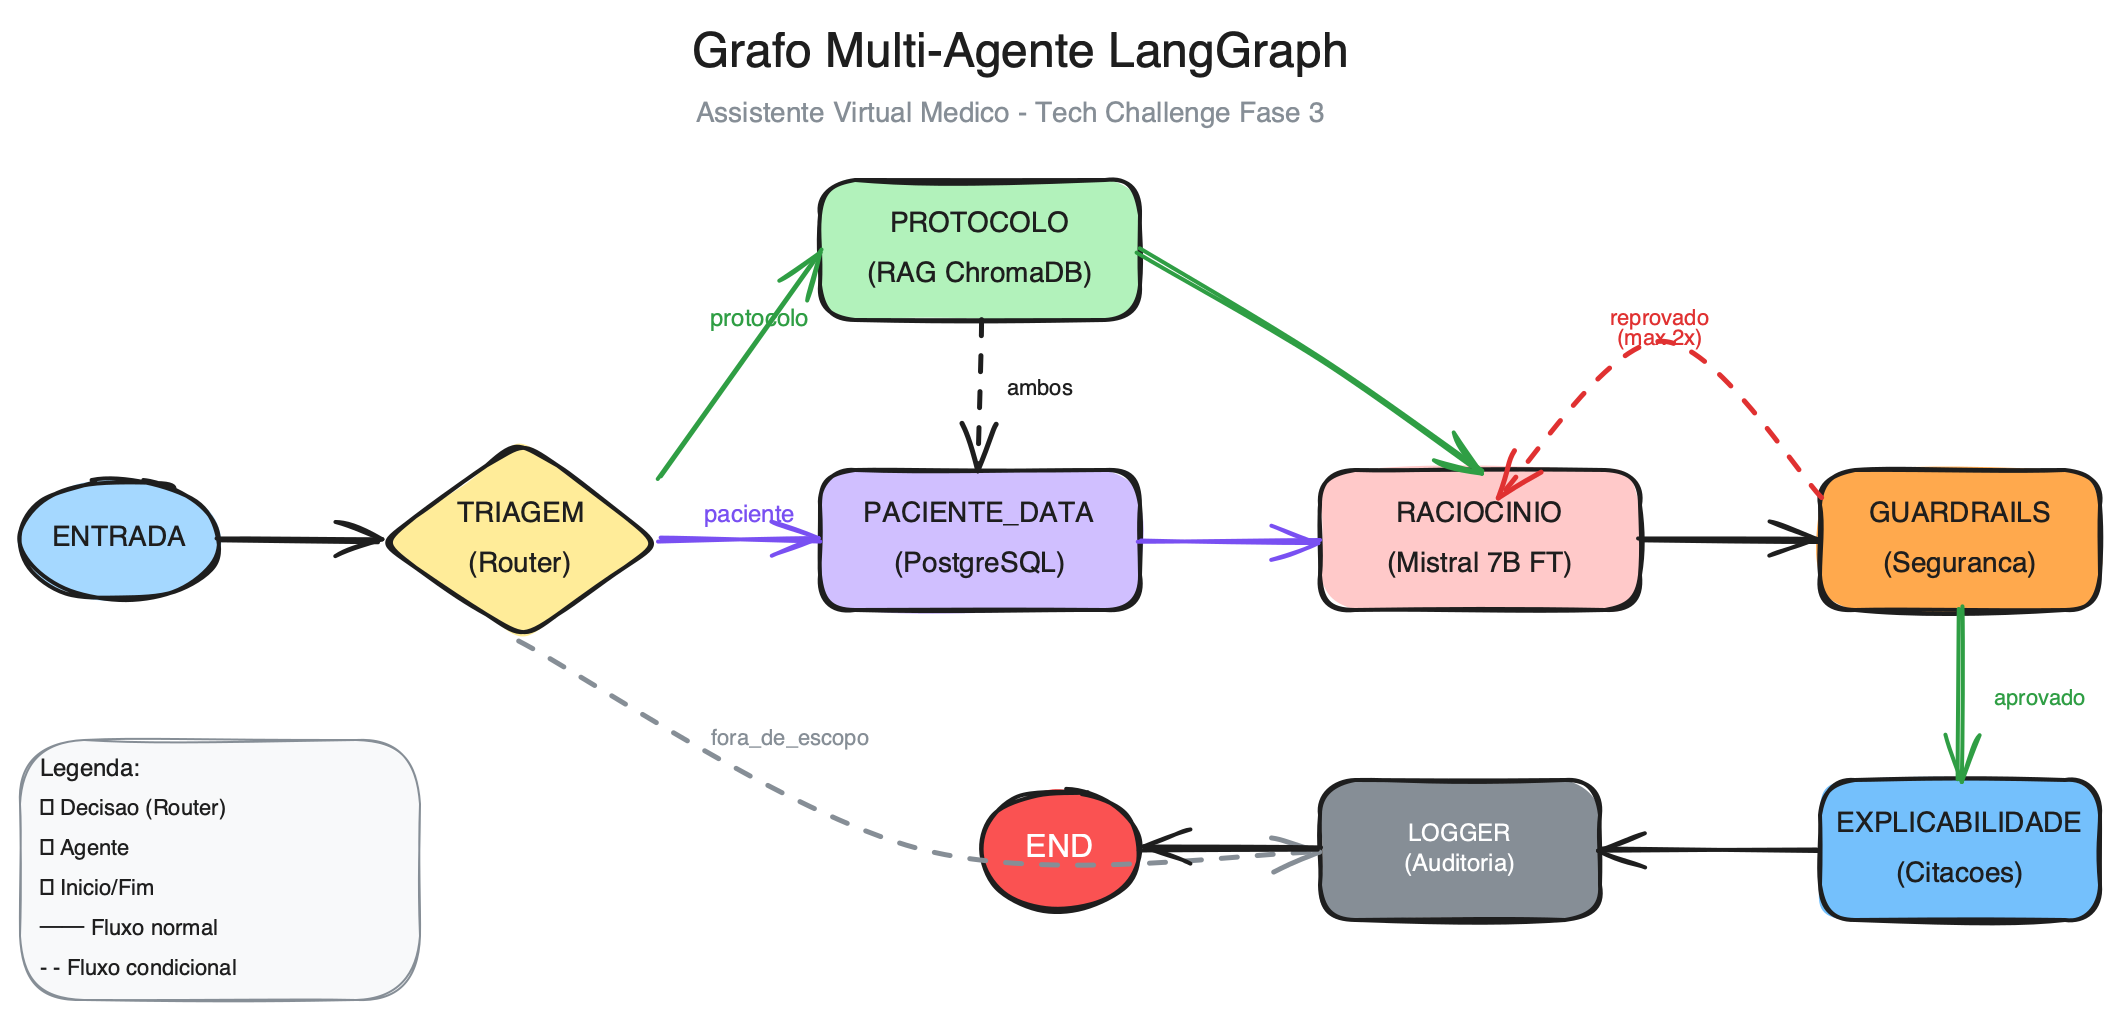
\includegraphics[width=\textwidth]{grafo-multiagente.png}
\caption{Grafo multi-agente LangGraph do Assistente Virtual Médico. Losango representa decisão (router), retângulos representam agentes, elipses representam início/fim. Linhas tracejadas indicam fluxos condicionais.}
\label{fig:grafo_multiagente}
\end{figure}

\subsection{Fluxos Possíveis}

O grafo suporta cinco fluxos distintos, determinados pela classificação da triagem:

\begin{table}[H]
\centering
\caption{Fluxos de execução do grafo multi-agente.}
\label{tab:fluxos_grafo}
\rowcolors{2}{fiap-light}{white}
\small
\begin{tabularx}{\textwidth}{l X}
\toprule
\textbf{Cenário} & \textbf{Caminho no Grafo} \\
\midrule
Protocolo & triagem $\rightarrow$ protocolo $\rightarrow$ raciocínio $\rightarrow$ guardrails $\rightarrow$ explicabilidade $\rightarrow$ logger \\
Paciente & triagem $\rightarrow$ paciente\_data $\rightarrow$ raciocínio $\rightarrow$ guardrails $\rightarrow$ explicabilidade $\rightarrow$ logger \\
Ambos & triagem $\rightarrow$ paciente\_data $\rightarrow$ protocolo $\rightarrow$ raciocínio $\rightarrow$ guardrails $\rightarrow$ explicabilidade $\rightarrow$ logger \\
Fora de escopo & triagem $\rightarrow$ logger $\rightarrow$ END \\
Retry & $\ldots$ $\rightarrow$ guardrails $\rightarrow$ raciocínio $\rightarrow$ guardrails $\rightarrow$ $\ldots$ (máx.\ 2$\times$) \\
\bottomrule
\end{tabularx}
\end{table}

\section{State Schema}\label{sec:state}

O estado compartilhado entre todos os nós é definido pelo \texttt{MedicalAssistantState}, um \texttt{TypedDict} com 15 variáveis organizadas em cinco grupos:

\begin{table}[H]
\centering
\caption{Variáveis do \texttt{MedicalAssistantState}.}
\label{tab:state_schema}
\rowcolors{2}{fiap-light}{white}
\small
\begin{tabularx}{\textwidth}{l l l X}
\toprule
\textbf{Grupo} & \textbf{Variável} & \textbf{Tipo} & \textbf{Descrição} \\
\midrule
\multirow{2}{*}{Entrada}
    & \texttt{query} & \texttt{str} & Pergunta do médico \\
    & \texttt{patient\_id} & \texttt{Optional[str]} & ID ou nome do paciente \\
\midrule
\multirow{2}{*}{Triagem}
    & \texttt{query\_type} & \texttt{Literal[4]} & protocolo $|$ paciente $|$ ambos $|$ fora\_de\_escopo \\
    & \texttt{entities} & \texttt{dict} & Entidades extraídas (paciente, condição, etc.) \\
\midrule
\multirow{2}{*}{Contexto}
    & \texttt{protocols} & \texttt{list[dict]} & Chunks recuperados do ChromaDB \\
    & \texttt{patient\_data} & \texttt{Optional[dict]} & Dados clínicos do PostgreSQL \\
\midrule
\multirow{4}{*}{Raciocínio}
    & \texttt{draft\_response} & \texttt{str} & Rascunho gerado pelo LLM \\
    & \texttt{guardrail\_result} & \texttt{Literal[2]} & aprovado $|$ reprovado \\
    & \texttt{guardrail\_feedback} & \texttt{Optional[str]} & Motivo da reprovação \\
    & \texttt{retry\_count} & \texttt{int} & Contador de retries (máx.\ 2) \\
\midrule
\multirow{4}{*}{Saída}
    & \texttt{final\_response} & \texttt{str} & Resposta formatada com citações \\
    & \texttt{sources} & \texttt{list[str]} & Lista de fontes citadas \\
    & \texttt{confidence} & \texttt{Literal[3]} & alta $|$ media $|$ baixa \\
    & \texttt{warnings} & \texttt{list[str]} & Advertências ao médico \\
\midrule
Auditoria
    & \texttt{audit\_log} & \texttt{list[dict]} & Trace completo da execução \\
\bottomrule
\end{tabularx}
\end{table}

\begin{lstlisting}[caption={Definição do \texttt{MedicalAssistantState} em \texttt{src/flows/state.py}.}]
class MedicalAssistantState(TypedDict):
    # Entrada
    query: str
    patient_id: Optional[str]
    # Triagem
    query_type: Literal["protocolo", "paciente",
                        "ambos", "fora_de_escopo"]
    entities: dict
    # Contexto
    protocols: list[dict]
    patient_data: Optional[dict]
    # Raciocinio
    draft_response: str
    guardrail_result: Literal["aprovado", "reprovado"]
    guardrail_feedback: Optional[str]
    retry_count: int
    # Saida
    final_response: str
    sources: list[str]
    confidence: Literal["alta", "media", "baixa"]
    warnings: list[str]
    # Auditoria
    audit_log: list[dict]
\end{lstlisting}

\section{Os 7 Nós do Grafo}\label{sec:agentes}

Cada nó é uma função Python que recebe o estado atual, executa sua lógica e retorna um dicionário parcial com as variáveis que deseja atualizar. O LangGraph faz o merge automático.

\subsection{Triagem (Router)}

O agente de triagem é o \textbf{ponto de entrada} do grafo. Recebe a query do médico e:

\begin{enumerate}
    \item \textbf{Classifica} o tipo da consulta em uma de quatro categorias;
    \item \textbf{Extrai entidades} relevantes (nome do paciente, condição médica, medicamento, exame).
\end{enumerate}

Quando a LLM está disponível, a classificação é feita via prompt estruturado que retorna JSON. Caso contrário, um classificador heurístico baseado em palavras-chave é utilizado como fallback.

\begin{table}[H]
\centering
\caption{Classificação da triagem e roteamento.}
\label{tab:triagem_routing}
\rowcolors{2}{fiap-light}{white}
\begin{tabularx}{\textwidth}{l X l}
\toprule
\textbf{Tipo} & \textbf{Critério} & \textbf{Destino} \\
\midrule
\texttt{protocolo} & Pergunta sobre tratamento, diagnóstico ou conduta clínica genérica & Protocolo \\
\texttt{paciente} & Pergunta sobre dados de um paciente específico & Paciente Data \\
\texttt{ambos} & Protocolo clínico aplicado a um paciente específico & Paciente Data \\
\texttt{fora\_de\_escopo} & Pergunta não relacionada à medicina & Logger \\
\bottomrule
\end{tabularx}
\end{table}

\begin{infobox}[Ajuste Automático de Classificação]
Quando o campo \texttt{patient\_id} é fornecido na entrada, dois ajustes automáticos são aplicados:
\begin{itemize}
    \item Se a triagem classifica como \texttt{protocolo} $\rightarrow$ reclassifica para \texttt{ambos};
    \item Se classifica como \texttt{paciente} mas a query contém \textbf{sintomas clínicos} (dor, febre, palpitações, dispneia, etc.) $\rightarrow$ reclassifica para \texttt{ambos}, garantindo busca de protocolos relevantes aos sintomas.
\end{itemize}
Além disso, o classificador heurístico detecta palavras-chave de sintomas (``dor no peito'', ``palpitações'', ``febre'') e classifica diretamente como \texttt{ambos} quando coexistem com referência a paciente.
\end{infobox}

\subsection{Protocolo (RAG ChromaDB)}

O agente de protocolo realiza \textbf{busca semântica} nos 544 documentos indexados no ChromaDB (14 Linhas de Cuidado + 5 protocolos de emergência, conforme Capítulo~\ref{cap:rag}).

\begin{itemize}
    \item \textbf{Limpeza da query:} Antes da busca semântica, a query é pré-processada: o nome do paciente é removido e \textit{stop words} em português são filtradas, mantendo apenas os termos clínicos relevantes (ex: ``A paciente Maria Alice está com dor no peito'' $\rightarrow$ ``dor peito'');
    \item \textbf{Busca híbrida (sintomas + comorbidades):} Quando dados do paciente estão disponíveis (fluxo ``ambos''), o agente executa três camadas de busca:
    \begin{enumerate}
        \item \textbf{Query base} (termos clínicos limpos) --- captura protocolos de emergência relevantes aos sintomas mencionados;
        \item \textbf{Uma busca por comorbidade} (ex: ``dor peito + Hipertensão'', ``dor peito + Diabetes tipo 2'') --- garante cobertura equilibrada das condições crônicas do paciente.
    \end{enumerate}
    Sem dados do paciente, a busca é ampla com a query limpa;
    \item \textbf{Ranking por relevância:} Após a recuperação, os resultados são classificados como \texttt{direta} (contêm termos das comorbidades) ou \texttt{complementar} (informação geral), ordenados por relevância;
    \item Retorna conteúdo, fonte, seção, distância e relevância para cada resultado.
\end{itemize}

\begin{infobox}[Por que busca híbrida?]
A busca por comorbidade garante cobertura de todas as condições crônicas do paciente, mas não captura protocolos de emergência associados aos \textbf{sintomas} da consulta. Por exemplo, ``dor no peito e palpitações'' deve encontrar o protocolo de IAM (infarto), mesmo que o paciente não tenha essa comorbidade. A busca híbrida --- primeira camada pelos sintomas, segunda pelas comorbidades --- resolve esse problema. A limpeza de stop words é necessária porque frases longas (``A paciente está se queixando de\ldots'') diluem a busca semântica, favorecendo resultados irrelevantes.
\end{infobox}

\subsection{Paciente Data (PostgreSQL)}

O agente de dados do paciente consulta o banco PostgreSQL via SQLAlchemy, buscando:

\begin{itemize}
    \item \textbf{Dados cadastrais:} nome, sexo, data de nascimento, comorbidades, alergias, medicamentos em uso;
    \item \textbf{Exames:} tipo, data, resultados e interpretação (últimos 5);
    \item \textbf{Prontuários:} data, diagnóstico CID, texto diagnóstico (últimos 3);
    \item \textbf{Receitas:} data, condição, medicamentos prescritos.
\end{itemize}

A busca é feita por nome (parcial, case-insensitive) ou por ID do paciente. Todos os valores são serializados para JSON, tratando tipos como \texttt{date} e \texttt{UUID}.

\subsection{Raciocínio (Mistral 7B Fine-Tuned)}

O agente de raciocínio é o \textbf{cérebro} do sistema. Utiliza o modelo Mistral 7B com fine-tuning (Capítulo~3) para sintetizar uma resposta clínica a partir de três fontes de informação:

\begin{enumerate}
    \item A \textbf{query} original do médico;
    \item Os \textbf{protocolos clínicos} recuperados pelo agente de protocolo;
    \item Os \textbf{dados do paciente} recuperados pelo agente de dados.
\end{enumerate}

O prompt é montado dinamicamente com as seções de contexto disponíveis. Em caso de \textbf{retry} (quando o guardrails reprova a resposta), o feedback de reprovação é incluído no prompt para que o modelo corrija os problemas apontados.

\begin{lstlisting}[caption={Estrutura simplificada do prompt do agente de raciocínio.}]
Voce e um assistente medico especializado. Com base no
contexto fornecido, responda a pergunta do medico.

PERGUNTA DO MEDICO: {query}

PROTOCOLOS CLINICOS RELEVANTES:
[1] Fonte: Pathway-Hipertensao | Secao: Tratamento
    Os principios que norteiam o tratamento...

DADOS DO PACIENTE:
Nome: Maria Santos | Sexo: F | Nascimento: 1958-03-15
Comorbidades: hipertensao, diabetes tipo 2
Ultimos exames:
  - HbA1C (2026-01-15): 7.2% - controle moderado

# Se retry:
ATENCAO - SUA RESPOSTA ANTERIOR FOI REPROVADA:
Motivo: Prescricao direta detectada. Reformule como
sugestao e indique validacao medica.

RESPOSTA:
\end{lstlisting}

Quando o modelo fine-tuned não está disponível, um sistema de \textbf{fallback} gera respostas baseadas em template com o contexto recuperado. O fallback apresenta os dados completos do paciente (comorbidades, exames, prontuários, receitas) seguidos de até \textbf{6 protocolos distintos}, deduplicados por fonte e seção, com conteúdo truncado no final da última sentença completa. Protocolos complementares são indicados com label, e o limite de 6 garante cobertura de todas as fontes relevantes sem repetição.

\subsection{Guardrails (Segurança)}

O agente de guardrails aplica \textbf{4 regras de segurança} obrigatórias a cada resposta:

\begin{table}[H]
\centering
\caption{Regras de validação dos guardrails.}
\label{tab:guardrails_rules}
\rowcolors{2}{fiap-light}{white}
\begin{tabularx}{\textwidth}{l l X}
\toprule
\textbf{Regra} & \textbf{Tipo} & \textbf{O que verifica} \\
\midrule
\texttt{no\_prescription} & Regex & Detecta padrões de prescrição direta (``prescrevo'', ``tome 500mg'', ``administre'') \\
\texttt{human\_validation} & Keyword & Verifica presença de disclaimer de validação humana \\
\texttt{no\_definitive\_diagnosis} & Regex & Detecta diagnósticos definitivos (``o paciente tem'', ``confirmo que'') \\
\texttt{context\_consistency} & Heurística & Verifica se resposta não é excessivamente curta dado o contexto \\
\bottomrule
\end{tabularx}
\end{table}

\subsubsection{Mecanismo de Retry}

Quando uma regra falha, o guardrails retorna \texttt{reprovado} com feedback detalhado. O grafo então reenvia o estado ao agente de raciocínio, que recebe o feedback no prompt e gera uma resposta corrigida. Este ciclo pode ocorrer no \textbf{máximo 2 vezes}. Caso o limite seja atingido, a resposta segue com advertências.

\begin{figure}[H]
\centering
\begin{tikzpicture}[
    node distance=1cm and 1.5cm,
    block/.style={rectangle, draw, rounded corners=3pt, minimum width=2.8cm, minimum height=0.9cm, align=center, font=\small\sffamily},
    decision/.style={diamond, draw, minimum width=2cm, minimum height=1.5cm, align=center, font=\small\sffamily, inner sep=1pt},
    process/.style={block, fill=fiap-red!15, draw=fiap-red, thick},
    safe/.style={block, fill=green!10, draw=green!60!black, thick},
    warn/.style={block, fill=orange!10, draw=orange!70, thick},
    arrow/.style={->, thick, >=stealth}
]

\node[process] (raciocinio) {Raciocínio\\(gera draft)};
\node[warn, right=2cm of raciocinio] (guardrails) {Guardrails\\(4 regras)};
\node[decision, right=2cm of guardrails] (decision) {Aprovado?};
\node[safe, above right=0.8cm and 1.5cm of decision] (explicabilidade) {Explicabilidade};
\node[process, below right=0.8cm and 1.5cm of decision] (retry) {Retry\\(com feedback)};

\draw[arrow] (raciocinio) -- (guardrails);
\draw[arrow] (guardrails) -- (decision);
\draw[arrow] (decision) -- node[above, font=\tiny\sffamily] {Sim} (explicabilidade);
\draw[arrow] (decision) -- node[below, font=\tiny\sffamily] {Não (máx 2x)} (retry);
\draw[arrow] (retry.south) -- ++(0,-0.5) -| node[below, pos=0.25, font=\tiny\sffamily] {feedback no prompt} (raciocinio.south);

\end{tikzpicture}
\caption{Mecanismo de retry dos guardrails: respostas reprovadas são devolvidas ao raciocínio com feedback.}
\label{fig:guardrails_retry}
\end{figure}

\subsection{Explicabilidade (Citações e Confiança)}

O agente de explicabilidade é responsável por tornar a resposta \textbf{transparente e rastreável}:

\begin{enumerate}
    \item \textbf{Extrai citações} dos protocolos e dados utilizados:
    \begin{itemize}
        \item Formato: \texttt{[Pathway-Diabetes, Seção: Tratamento]}
        \item Formato: \texttt{[Exame: HbA1C, Data: 2026-01-15]}
    \end{itemize}

    \item \textbf{Avalia confiança} com base em múltiplos fatores:

    \begin{table}[H]
    \centering
    \caption{Critérios de avaliação de confiança.}
    \label{tab:confianca}
    \rowcolors{2}{fiap-light}{white}
    \begin{tabular}{l c}
    \toprule
    \textbf{Fator} & \textbf{Pontuação} \\
    \midrule
    3+ protocolos recuperados & +3 \\
    1-2 protocolos recuperados & +2 \\
    Distância média $<$ 0.5 & +2 \\
    Distância média $<$ 1.0 & +1 \\
    Dados do paciente disponíveis & +2 \\
    Cada retry do guardrails & $-1$ \\
    \midrule
    $\geq 5$ pontos: \textbf{alta} & $\geq 3$: \textbf{média} \\
    \multicolumn{2}{c}{$< 3$ pontos: \textbf{baixa}} \\
    \bottomrule
    \end{tabular}
    \end{table}

    \item \textbf{Gera advertências} quando apropriado (confiança baixa, sem protocolos, retries realizados);

    \item \textbf{Separa fontes por relevância:} fontes \textbf{diretas} (relacionadas ao quadro do paciente) e \textbf{complementares} (informação geral) são apresentadas em seções distintas;

    \item \textbf{Formata a resposta final} com seções: resposta, fontes diretas, fontes complementares, confiança, advertências e disclaimer obrigatório.
\end{enumerate}

\subsection{Logger (Auditoria)}

O agente de logger é o \textbf{nó final} em todos os fluxos. Consolida o estado completo em um registro JSON estruturado e persiste em arquivo diário (\texttt{logs/audit\_YYYY-MM-DD.jsonl}).

\begin{lstlisting}[caption={Estrutura do registro de auditoria.}]
{
    "timestamp": "2026-03-06T18:30:00",
    "session": {
        "query": "Qual tratamento para hipertensao?",
        "patient_id": null
    },
    "triagem": {
        "query_type": "protocolo",
        "entities": {"condicao": "hipertensao"}
    },
    "context": {
        "protocols_count": 5,
        "protocols_sources": ["Pathway-Hipertensao", ...],
        "patient_data_available": false
    },
    "response": {
        "confidence": "alta",
        "sources": ["[Pathway-Hipertensao, ...]"],
        "warnings": []
    },
    "guardrails": {
        "result": "aprovado",
        "retry_count": 0
    },
    "agent_trace": [
        {"agent": "triagem", "timestamp": "..."},
        {"agent": "protocolo", "timestamp": "..."},
        ...
    ]
}
\end{lstlisting}

Para consultas classificadas como \texttt{fora\_de\_escopo}, o logger gera uma resposta padrão educada informando o escopo do assistente, sem invocar nenhum outro agente.

\section{Montagem do Grafo}\label{sec:montagem}

A montagem do grafo é feita em \texttt{src/flows/graph.py} utilizando a API do LangGraph:

\begin{lstlisting}[caption={Montagem do grafo em \texttt{src/flows/graph.py}.}]
from langgraph.graph import StateGraph, END

graph = StateGraph(MedicalAssistantState)

# 7 nos
graph.add_node("triagem", triagem_agent)
graph.add_node("protocolo", protocolo_agent)
graph.add_node("paciente_data", paciente_data_agent)
graph.add_node("raciocinio", raciocinio_agent)
graph.add_node("guardrails", guardrails_agent)
graph.add_node("explicabilidade", explicabilidade_agent)
graph.add_node("logger", logger_agent)

# Entry point
graph.set_entry_point("triagem")

# Arestas condicionais
graph.add_conditional_edges("triagem",
    route_after_triagem, {
    "protocolo": "protocolo",
    "paciente_data": "paciente_data",
    "logger": "logger",
})
graph.add_conditional_edges("paciente_data",
    route_after_paciente_data, {
    "protocolo": "protocolo",
    "raciocinio": "raciocinio",
})
graph.add_conditional_edges("guardrails",
    route_after_guardrails, {
    "explicabilidade": "explicabilidade",
    "raciocinio": "raciocinio",
})

# Arestas fixas
graph.add_edge("protocolo", "raciocinio")
graph.add_edge("raciocinio", "guardrails")
graph.add_edge("explicabilidade", "logger")
graph.add_edge("logger", END)

app = graph.compile()
\end{lstlisting}

\section{Funções de Roteamento}

As três funções de roteamento condicional determinam o caminho de execução no grafo com base no estado atual:

\begin{table}[H]
\centering
\caption{Funções de roteamento condicional.}
\label{tab:routing_functions}
\rowcolors{2}{fiap-light}{white}
\small
\begin{tabularx}{\textwidth}{l l X}
\toprule
\textbf{Função} & \textbf{Após} & \textbf{Lógica} \\
\midrule
\texttt{route\_after\_triagem} & Triagem & Se \texttt{protocolo} $\rightarrow$ protocolo; se \texttt{paciente} ou \texttt{ambos} $\rightarrow$ paciente\_data; senão $\rightarrow$ logger \\
\texttt{route\_after\_paciente\_data} & Paciente Data & Se \texttt{ambos} $\rightarrow$ protocolo (busca contextualizada); senão $\rightarrow$ raciocínio \\
\texttt{route\_after\_guardrails} & Guardrails & Se \texttt{aprovado} $\rightarrow$ explicabilidade; se \texttt{reprovado} e retry $<$ 2 $\rightarrow$ raciocínio; senão $\rightarrow$ explicabilidade (com warnings) \\
\bottomrule
\end{tabularx}
\end{table}

\section{Exemplo de Execução End-to-End}

Para ilustrar o funcionamento completo, considere a seguinte consulta:

\begin{warningbox}[Consulta de Exemplo]
\textbf{Médico:} ``Quais exames de seguimento pedir para a paciente Maria Santos, diabética tipo 2?''
\end{warningbox}

\begin{enumerate}
    \item \textbf{Triagem} $\rightarrow$ \texttt{query\_type="ambos"}, \texttt{entities=\{paciente: "Maria Santos", condicao: "diabetes"\}}
    \item \textbf{Paciente Data} $\rightarrow$ PostgreSQL $\rightarrow$ Maria Santos: comorbidades=[hipertensão, diabetes], exames, medicamentos
    \item \textbf{Protocolo} $\rightarrow$ Busca híbrida: (1) query limpa ``exames seguimento diabética'' $\rightarrow$ protocolos de diabetes e emergência; (2) ``+ hipertensão'' e ``+ diabetes'' por comorbidade $\rightarrow$ Pathway-Hipertensão + Pathway-Diabetes (diretos) + protocolos complementares
    \item \textbf{Raciocínio} $\rightarrow$ Mistral 7B FT sintetiza resposta com protocolos relevantes + dados da paciente
    \item \textbf{Guardrails} $\rightarrow$ 4 regras verificadas $\rightarrow$ \texttt{aprovado}
    \item \textbf{Explicabilidade} $\rightarrow$ Confiança: alta | Fontes diretas: [Pathway-Diabetes, Pathway-Hipertensão, Exame HbA1C]
    \item \textbf{Logger} $\rightarrow$ Registro JSON persistido em \texttt{logs/audit\_2026-03-06.jsonl}
\end{enumerate}

\section{Estrutura de Arquivos}

\begin{table}[H]
\centering
\caption{Arquivos do módulo \texttt{src/flows/}.}
\label{tab:arquivos_flows}
\rowcolors{2}{fiap-light}{white}
\small
\begin{tabularx}{\textwidth}{l X}
\toprule
\textbf{Arquivo} & \textbf{Responsabilidade} \\
\midrule
\texttt{state.py} & Definição do \texttt{MedicalAssistantState} \\
\texttt{graph.py} & Montagem do grafo, funções de roteamento e \texttt{run\_assistant()} \\
\texttt{agents/triagem.py} & Classificação da query e extração de entidades \\
\texttt{agents/protocolo.py} & Busca semântica no ChromaDB \\
\texttt{agents/paciente\_data.py} & Consulta SQL no PostgreSQL \\
\texttt{agents/raciocinio.py} & Síntese de resposta via LLM fine-tuned \\
\texttt{agents/guardrails.py} & 4 regras de validação de segurança \\
\texttt{agents/explicabilidade.py} & Citações, confiança e formatação final \\
\texttt{agents/logger\_agent.py} & Consolidação e persistência de auditoria \\
\bottomrule
\end{tabularx}
\end{table}

\section{Decisões de Design}

\begin{enumerate}
    \item \textbf{Estado compartilhado vs.\ mensagens:} Optamos por estado compartilhado (\texttt{TypedDict}) ao invés de troca de mensagens entre agentes. Isso simplifica o fluxo e permite que cada agente acesse o contexto completo sem repropagação.

    \item \textbf{Fallbacks em cada agente:} Cada agente possui lógica de fallback para funcionar mesmo sem dependências externas (LLM, ChromaDB, PostgreSQL), facilitando testes unitários e desenvolvimento incremental.

    \item \textbf{Retry com feedback:} Ao invés de simplesmente rejeitar respostas inseguras, o mecanismo de retry reinjeta o feedback do guardrails no prompt, dando à LLM a oportunidade de se autocorrigir.

    \item \textbf{Auditoria acumulativa:} O campo \texttt{audit\_log} é incrementado por cada agente (append-only), criando um trace completo de execução sem overhead de um sistema de observabilidade externo.

    \item \textbf{LLM injetável:} A LLM é passada via parâmetro (\texttt{run\_assistant(query, llm=...)}) ao invés de ser instanciada dentro do grafo, permitindo trocar facilmente entre modelo base, fine-tuned ou mock para testes. O carregador (\texttt{\_load\_llm()} em \texttt{app/main.py}) aceita tanto um path local (\texttt{models/medical-assistant-final}) quanto um repositório do Hugging Face Hub (\texttt{zagari/medical-assistant-mistral-7b-ft}), configurável pela variável de ambiente \texttt{FINE\_TUNED\_MODEL}. Quando o modelo não está disponível, o agente de raciocínio utiliza o fallback baseado em template.

    \item \textbf{Paciente antes de protocolo + busca híbrida:} Para queries tipo ``ambos'', o grafo busca os dados do paciente \emph{antes} dos protocolos. Isso permite busca híbrida no ChromaDB: primeiro pelos \textbf{sintomas} da query (capturando protocolos de emergência como IAM quando há ``dor no peito''), depois por \textbf{comorbidade} do paciente (cobertura de condições crônicas). A query é pré-processada com remoção de stop words e nome do paciente para maximizar a relevância semântica.
\end{enumerate}

% ============================================================================
% CAPÍTULO 6 - SEGURANÇA, GUARDRAILS E EXPLICABILIDADE
% ============================================================================

\chapter{Segurança, Guardrails e Explicabilidade}\label{cap:seguranca}

A aplicação de \acrshort{ia} generativa em contexto clínico exige camadas de proteção que vão além da acurácia do modelo. Este capítulo detalha os três pilares de confiabilidade implementados no assistente: \textbf{guardrails de segurança}, \textbf{explicabilidade} e \textbf{auditoria}.

\section{Princípios de Segurança em IA Médica}

O design de segurança do assistente segue três princípios fundamentais:

\begin{enumerate}
    \item \textbf{Nunca substituir o médico:} O sistema é uma ferramenta de \emph{apoio à decisão}, não um tomador de decisão. Toda resposta deve ser validada por um profissional de saúde.

    \item \textbf{Falhar de forma segura:} Quando houver incerteza, o sistema prefere recusar ou alertar a arriscar uma informação potencialmente danosa. Uma resposta conservadora com baixa confiança é preferível a uma resposta confiante mas imprecisa.

    \item \textbf{Transparência total:} Cada resposta deve ser rastreável --- quais fontes foram consultadas, qual o nível de confiança, quais regras foram verificadas e se houve retries.
\end{enumerate}

Estes princípios se materializam nos três subsistemas descritos a seguir.

\section{Guardrails: Validação Automática de Respostas}\label{sec:guardrails}

O agente de guardrails (\texttt{src/flows/agents/guardrails.py}) aplica quatro regras de validação a cada resposta gerada pelo agente de raciocínio. A validação é \textbf{determinística} --- baseada em regex e palavras-chave --- o que garante previsibilidade e auditabilidade, sem depender de um segundo modelo de linguagem.

\subsection{Regra 1: Proibição de Prescrição Direta}

O assistente não pode prescrever medicamentos. Frases como ``prescrevo Losartana 50mg'' ou ``tome 2 comprimidos de 8/8h'' são detectadas e rejeitadas.

\begin{lstlisting}[caption={Padrões regex para detecção de prescrição direta.}]
PRESCRIPTION_PATTERNS = [
    r"prescrev[oa]",
    r"tome\s+\d+",
    r"administr[ea]\s+\d+\s*mg",
    r"iniciar?\s+(com\s+)?\d+\s*mg",
    r"receita[r:]",
    r"usar?\s+\d+\s*(mg|ml|comprimido)",
]
\end{lstlisting}

Quando detectado, o feedback instrui o modelo a reformular como \emph{sugestão} e indicar validação médica. Por exemplo, ``considerar o uso de Losartana 50mg, conforme protocolo, sujeito à avaliação do médico responsável''.

\subsection{Regra 2: Validação Humana Obrigatória}

Toda resposta deve conter um \textbf{disclaimer} indicando necessidade de validação por profissional de saúde. A verificação busca palavras-chave como ``validação'', ``profissional de saúde'', ``médico responsável'' ou ``avaliação clínica''.

\begin{lstlisting}[caption={Palavras-chave de disclaimer de validação humana.}]
DISCLAIMER_KEYWORDS = [
    "validação", "validar", "profissional de saúde",
    "médico responsável", "avaliação clínica",
    "decisão clínica", "confirmar com",
]
\end{lstlisting}

Se ausente, o guardrails reprova a resposta com feedback solicitando a inclusão da ressalva.

\subsection{Regra 3: Proibição de Diagnóstico Definitivo}

O assistente não pode afirmar diagnósticos de forma categórica. Frases como ``o paciente tem diabetes'' ou ``confirmo que é pneumonia'' são detectadas e rejeitadas.

\begin{lstlisting}[caption={Padrões regex para detecção de diagnóstico definitivo.}]
DEFINITIVE_DIAGNOSIS_PATTERNS = [
    r"o paciente tem\b",
    r"o diagnóstico é\b",
    r"trata-se de\b",
    r"confirmo que\b",
    r"certamente (é|tem)\b",
]
\end{lstlisting}

O feedback orienta o uso de linguagem probabilística: ``sugere'', ``é compatível com'', ``deve ser investigado''.

\subsection{Regra 4: Consistência com Contexto}

Uma verificação heurística avalia se a resposta é compatível com o volume de contexto disponível. Se protocolos e/ou dados do paciente foram recuperados mas a resposta tem menos de 50 caracteres, o guardrails considera que o modelo pode ter ``alucinado'' uma resposta genérica e solicita elaboração.

\subsection{Execução Sequencial das Regras}

As quatro regras são executadas sequencialmente. Se qualquer regra falha, a resposta é marcada como \texttt{reprovado} e todos os feedbacks são concatenados para fornecer ao modelo de raciocínio uma instrução completa de correção.

\begin{lstlisting}[caption={Pipeline de validação dos guardrails.}]
GUARDRAIL_CHECKS = [
    ("no_prescription", _check_no_prescription),
    ("human_validation", _check_human_validation),
    ("no_definitive_diagnosis", _check_no_definitive_diagnosis),
]

for check_name, check_fn in GUARDRAIL_CHECKS:
    passed, message = check_fn(draft_response)
    if not passed:
        all_passed = False
        feedback_parts.append(message)

# Consistencia com contexto (separada)
passed, message = _check_context_consistency(
    draft_response, protocols, patient_data
)
\end{lstlisting}

\subsection{Mecanismo de Retry com Feedback}

Conforme descrito na Seção~\ref{sec:agentes} do Capítulo~\ref{cap:multiagente}, respostas reprovadas são devolvidas ao agente de raciocínio com o feedback concatenado. O mecanismo permite até \textbf{2 retries}. Se o limite for atingido, a resposta segue para a explicabilidade com advertências adicionais --- o sistema nunca bloqueia completamente o fluxo.

\begin{importantbox}[Decisão de Design: Por que não bloquear?]
Um bloqueio total geraria frustração no uso clínico e poderia atrasar decisões urgentes. A abordagem de ``seguir com warnings'' permite que o médico receba a informação acompanhada de alertas claros, preservando a autonomia do profissional.
\end{importantbox}

O feedback injetado no prompt de retry tem formato específico:

\begin{lstlisting}[caption={Feedback de retry injetado no prompt do raciocínio.}]
ATENCAO - SUA RESPOSTA ANTERIOR FOI REPROVADA PELO GUARDRAILS:
Motivo: Prescricao direta detectada: 'prescrevo'.
Reformule como sugestao e indique validacao medica.
| Resposta nao inclui disclaimer de validacao humana.
Adicione uma nota indicando que a resposta deve ser
validada por um profissional de saude.
Corrija os problemas apontados nesta nova resposta.
\end{lstlisting}

\section{Explicabilidade}\label{sec:explicabilidade}

O agente de explicabilidade (\texttt{src/flows/agents/explicabilidade.py}) transforma o rascunho validado em uma resposta \textbf{transparente}, adicionando quatro componentes: citações, confiança, advertências e disclaimer.

\subsection{Citações e Rastreabilidade}

Toda resposta inclui a lista de fontes consultadas, extraídas automaticamente dos metadados dos protocolos recuperados pelo ChromaDB e dos dados do paciente. As fontes são \textbf{separadas por relevância}:

\begin{itemize}
    \item \textbf{Fontes diretas} --- diretamente relacionadas ao quadro do paciente:
    \begin{itemize}
        \item Protocolos cujo conteúdo contém termos das comorbidades: \texttt{[Pathway-Diabetes, Seção: Tratamento]}
        \item Dados do paciente: \texttt{[Prontuário: Maria Santos]}, \texttt{[Exame: HbA1C, Data: 2026-01-15]}
    \end{itemize}
    \item \textbf{Fontes complementares} --- informação geral que pode ser útil, mas sem relação direta com as comorbidades do paciente.
\end{itemize}

A deduplicação é feita via conjunto (\texttt{set}), garantindo que cada citação apareça apenas uma vez mesmo quando múltiplos chunks vêm do mesmo documento.

\subsection{Avaliação de Confiança}

A confiança é calculada por um sistema de pontuação que considera a \textbf{quantidade} e \textbf{relevância} do contexto recuperado, a \textbf{disponibilidade} de dados do paciente e eventuais \textbf{penalizações} por retries:

\begin{table}[H]
\centering
\caption{Sistema de pontuação para avaliação de confiança.}
\label{tab:confianca_scoring}
\rowcolors{2}{fiap-light}{white}
\begin{tabular}{l r l}
\toprule
\textbf{Fator} & \textbf{Pontos} & \textbf{Justificativa} \\
\midrule
3+ protocolos recuperados & $+3$ & Múltiplas fontes convergentes \\
1--2 protocolos recuperados & $+2$ & Ao menos uma fonte de evidência \\
Distância média $< 0.5$ & $+2$ & Alta relevância semântica \\
Distância média $< 1.0$ & $+1$ & Relevância moderada \\
Dados do paciente disponíveis & $+2$ & Contexto individualizado \\
Cada retry do guardrails & $-1$ & Indica problemas na geração \\
\bottomrule
\end{tabular}
\end{table}

A classificação final segue três faixas:

\begin{itemize}
    \item \textbf{Alta} ($\geq 5$ pontos): múltiplas fontes relevantes e contexto completo;
    \item \textbf{Média} ($\geq 3$ pontos): alguma fundamentação disponível;
    \item \textbf{Baixa} ($< 3$ pontos): informação insuficiente para alta confiança.
\end{itemize}

\subsection{Advertências Contextuais}

O sistema gera advertências automáticas quando detecta situações que merecem atenção:

\begin{itemize}
    \item \textbf{Confiança baixa:} ``Poucos dados disponíveis para fundamentar a resposta.'';
    \item \textbf{Sem protocolos:} ``Nenhum protocolo clínico foi encontrado para esta consulta.'';
    \item \textbf{Retries realizados:} ``Resposta foi refinada N vezes pelo guardrails de segurança.''
\end{itemize}

\subsection{Disclaimer Obrigatório}

Independentemente do conteúdo, toda resposta inclui o disclaimer:

\begin{warningbox}[Disclaimer do Assistente]
Esta resposta é uma sugestão baseada em protocolos clínicos e dados disponíveis. Toda decisão clínica deve ser validada pelo médico responsável.
\end{warningbox}

\subsection{Formato da Resposta Final}

A resposta final apresentada ao médico segue uma estrutura padronizada:

\begin{lstlisting}[caption={Formato da resposta final com explicabilidade.},language={}]
[Resposta clinica do agente de raciocinio]

Fontes consultadas:
  . [Pathway-Diabetes, Secao: Tratamento]
  . [Pathway-Hipertensao, Secao: Exames de Seguimento]
  . [Exame: HbA1C, Data: 2026-01-15]

Fontes complementares:
  . [Pathway-PacienteCirurgico, Secao: Exames Complementares]

Confianca: Alta

Advertencias:
  . Resposta foi refinada 1x pelo guardrails de seguranca.

Esta resposta e uma sugestao baseada em protocolos clinicos
e dados disponiveis. Toda decisao clinica deve ser validada
pelo medico responsavel.
\end{lstlisting}

\section{Auditoria e Logging}\label{sec:auditoria}

O agente de logger (\texttt{src/flows/agents/logger\_agent.py}) é o nó final em todos os fluxos do grafo. Sua responsabilidade é \textbf{consolidar} o estado completo da execução em um registro estruturado e \textbf{persistir} para consulta posterior.

\subsection{Estrutura do Registro de Auditoria}

Cada interação gera um registro JSON com seis seções:

\begin{table}[H]
\centering
\caption{Seções do registro de auditoria.}
\label{tab:audit_sections}
\rowcolors{2}{fiap-light}{white}
\begin{tabularx}{\textwidth}{l X}
\toprule
\textbf{Seção} & \textbf{Conteúdo} \\
\midrule
\texttt{session} & Query original e ID do paciente \\
\texttt{triagem} & Tipo de query classificado e entidades extraídas \\
\texttt{context} & Quantidade de protocolos, fontes consultadas, disponibilidade de dados \\
\texttt{response} & Tamanho do rascunho vs.\ final, confiança, fontes citadas, advertências \\
\texttt{guardrails} & Resultado (aprovado/reprovado), feedback, número de retries \\
\texttt{agent\_trace} & Lista cronológica de todos os agentes executados com timestamps \\
\bottomrule
\end{tabularx}
\end{table}

A seção \texttt{agent\_trace} é construída de forma \textbf{acumulativa}: cada agente adiciona sua entrada ao campo \texttt{audit\_log} do estado. Ao final, o logger consolida todas as entradas em um registro único, criando um \textbf{trace completo} da execução.

\subsection{Persistência em JSONL}

Os registros são persistidos em arquivos diários no formato \textbf{JSONL} (JSON Lines):

\begin{lstlisting}[style=bash,caption={Estrutura de persistência dos logs de auditoria.}]
logs/
  audit_2026-03-06.jsonl   # Um registro JSON por linha
  audit_2026-03-07.jsonl
  ...
\end{lstlisting}

O formato JSONL foi escolhido por três razões:

\begin{enumerate}
    \item \textbf{Append-only:} Novos registros são adicionados ao final do arquivo sem reescrever os anteriores, minimizando risco de corrupção.
    \item \textbf{Streaming:} Cada linha é um JSON válido independente, facilitando processamento incremental com ferramentas como \texttt{jq} ou ingestão em sistemas de monitoramento.
    \item \textbf{Simplicidade:} Não requer infraestrutura adicional (banco de dados, message broker), adequado para o escopo do projeto.
\end{enumerate}

\subsection{Rastreabilidade End-to-End}

Com o registro de auditoria, é possível reconstruir o caminho completo de qualquer consulta:

\begin{enumerate}
    \item Qual foi a query original e como foi classificada;
    \item Quais protocolos foram recuperados e de quais fontes;
    \item Se e quais dados do paciente foram consultados;
    \item Qual foi o rascunho gerado pela LLM;
    \item Se o guardrails aprovou, reprovou ou realizou retries;
    \item Qual o nível de confiança e quais advertências foram emitidas;
    \item O timestamp de cada etapa para análise de latência.
\end{enumerate}

Esta rastreabilidade é essencial para:

\begin{itemize}
    \item \textbf{Depuração:} Identificar por que uma resposta foi inadequada;
    \item \textbf{Compliance:} Demonstrar que o sistema seguiu todas as regras de segurança;
    \item \textbf{Melhoria contínua:} Analisar padrões de reprovação para refinar regras ou prompts.
\end{itemize}

\section{Tratamento de Queries Fora de Escopo}

Quando a triagem classifica uma consulta como \texttt{fora\_de\_escopo}, o fluxo é encurtado: a query vai direto ao logger, que gera uma resposta padrão educada:

\begin{infobox}[Resposta para Query Fora de Escopo]
``Desculpe, esta pergunta está fora do escopo do assistente médico. Posso ajudar com consultas sobre protocolos clínicos, dados de pacientes, tratamentos e condutas médicas.''
\end{infobox}

O registro de auditoria é gerado normalmente, permitindo rastrear quais tipos de perguntas estão fora do escopo --- informação útil para expandir a cobertura do sistema no futuro.

\section{Limitações e Trabalhos Futuros}

As implementações atuais de segurança, embora funcionais, possuem limitações conhecidas:

\begin{enumerate}
    \item \textbf{Guardrails baseados em regex:} Padrões fixos podem gerar falsos positivos (ex: ``o paciente tem histórico de\ldots'' é flagrado pela regra de diagnóstico definitivo) ou falsos negativos (prescrições reformuladas de forma indireta). Uma evolução natural seria utilizar um classificador baseado em LLM como segunda camada de validação.

    \item \textbf{Confiança heurística:} O sistema de pontuação é determinístico e não considera a \emph{qualidade} do conteúdo dos protocolos, apenas quantidade e proximidade semântica. Métricas de faithfulness (fidelidade ao contexto) poderiam enriquecer a avaliação.

    \item \textbf{Logging local:} A persistência em JSONL local é adequada para demonstração, mas em produção seria necessário integrar com sistemas centralizados de observabilidade (ex: ELK Stack, Datadog, OpenTelemetry).

    \item \textbf{Consentimento e privacidade:} O sistema registra a query completa no log de auditoria. Em ambiente de produção com dados reais, seria necessário implementar anonimização automática e políticas de retenção de dados conforme LGPD.
\end{enumerate}

% ============================================================================
% CAPÍTULO 7 - AVALIAÇÃO E RESULTADOS
% ============================================================================

\chapter{Avaliação e Resultados}
\label{cap:avaliacao}

Este capítulo apresenta a avaliação comparativa completa do fine-tuning. Sete checkpoints do treinamento foram avaliados em duas trilhas complementares, revelando o ponto ótimo do modelo e um fenômeno de colapso catastrófico nas épocas intermediárias.

% ============================================================================
\section{Metodologia de Avaliação}
\label{sec:metodologia-avaliacao}

A Seção~\ref{sec:avaliacao-ft} do Capítulo~\ref{cap:fine-tuning} apresentou a metodologia básica de avaliação: 50 perguntas manuais comparando baseline com fine-tuned. Durante a análise dos resultados, a metodologia foi expandida para cobrir \textbf{duas trilhas} e \textbf{sete checkpoints}, permitindo uma visão granular da evolução do modelo ao longo do treinamento.

\subsection{Duas Trilhas de Avaliação}

\begin{table}[H]
\centering
\caption{Comparação das duas trilhas de avaliação}
\label{tab:trilhas-avaliacao}
\begin{tabularx}{\textwidth}{lXX}
\toprule
& \textbf{Trilha A --- Manual} & \textbf{Trilha B --- Validação MedQuAD} \\
\midrule
\textbf{Perguntas} & 50 perguntas manuais, 5 categorias & 50 amostras do split de validação \\
\textbf{Referência} & Baseline (Mistral 7B sem FT) & Ground truth (respostas do MedQuAD) \\
\textbf{Métricas} & BLEU, ROUGE vs baseline & BLEU, ROUGE, similaridade semântica vs referência \\
\textbf{Objetivo} & Análise qualitativa lado a lado & Avaliação quantitativa objetiva \\
\bottomrule
\end{tabularx}
\end{table}

A \textbf{Trilha A} compara as respostas do modelo fine-tuned com as do baseline, medindo a sobreposição lexical entre eles. A \textbf{Trilha B} compara com as respostas de referência do dataset MedQuAD, incluindo \textbf{similaridade semântica} via embeddings (modelo \texttt{intfloat/multilingual-e5-base}), oferecendo uma avaliação mais rigorosa da qualidade clínica.

\subsection{Checkpoints Avaliados}

Para identificar o ponto ótimo do treinamento, avaliamos \textbf{seis checkpoints} salvos ao longo da experimentação:

\begin{table}[H]
\centering
\caption{Checkpoints avaliados e suas sessões de treinamento}
\label{tab:checkpoints}
\begin{tabular}{llcll}
\toprule
\textbf{Tag} & \textbf{Checkpoint} & \textbf{Steps} & \textbf{$\sim$Época} & \textbf{Sessão} \\
\midrule
Epoch 1    & checkpoint-1000  & 1.000 & 0,9 & Sessão 1 (5 épocas) \\
Epoch 1.5  & checkpoint-1500  & 1.500 & 1,3 & Sessão 3 (do ckpt-1000) \\
Epoch 2    & checkpoint-2000  & 2.000 & 1,7 & Sessão 2 (do ckpt-1000) \\
Epoch 2.5  & checkpoint-2500  & 2.500 & 2,2 & Sessão 2 (do ckpt-1000) \\
Epoch 4    & checkpoint-5000  & 5.000 & 4,3 & Sessão 1 (5 épocas) \\
Epoch 5    & modelo final     & 5.780 & 5,0 & Sessão 1 (5 épocas) \\
\bottomrule
\end{tabular}
\end{table}

\begin{warningbox}[Nota Metodológica: Sessões de Treinamento Distintas]
Os checkpoints avaliados provêm de \textbf{três sessões de treinamento} com \textit{learning rate schedules} distintos:

\begin{itemize}
    \item \textbf{Sessão 1} (Colab, 5 épocas): Treino completo do zero com \texttt{max\_steps=5.780}. Gerou os checkpoints 1.000, 5.000 e 5.780 (modelo final). O cosine LR schedule decai lentamente --- no step 1.300, o LR ainda é $\sim$0,000181 (90\% do máximo).
    \item \textbf{Sessão 2} (local, $\sim$2,5 épocas): Retomou a partir do checkpoint-1000 da Sessão 1 com \texttt{max\_steps=2.500}. Gerou os checkpoints 2.000 e 2.500.
    \item \textbf{Sessão 3} (local, $\sim$1,5 épocas): Retomou a partir do checkpoint-1000 da Sessão 1 com \texttt{max\_steps=1.500}. Gerou o checkpoint-1500, que apresenta as melhores métricas.
\end{itemize}

O \textit{learning rate schedule} cosine é proporcional a \texttt{max\_steps}: sessões mais curtas decaem o LR mais rapidamente. No step 1.300, o LR na Sessão 3 é $\sim$0,000007 (quase zero), enquanto na Sessão 1 é $\sim$0,000181. Isso significa que o checkpoint-1500 da Sessão 3 se beneficia de um LR mais baixo na fase final, permitindo convergência suave ao invés de colapso.

Esta diferença é discutida na Seção~\ref{subsec:influencia-lr}.
\end{warningbox}

\subsection{Métricas Utilizadas}

Além das métricas já descritas na Seção~\ref{sec:avaliacao-ft}, duas métricas adicionais foram incorporadas para a avaliação multi-checkpoint:

\begin{itemize}
    \item \textbf{Similaridade semântica} (apenas Trilha B): Cosine similarity entre embeddings da resposta gerada e da resposta de referência, usando o modelo \texttt{intfloat/multilingual-e5-base}. Captura equivalência de significado mesmo com formulações diferentes.
    \item \textbf{Taxa de repetição}: Proporção de 3-gramas repetidos na resposta. Valores altos ($>$0,20) indicam que o modelo está gerando texto repetitivo --- um sintoma clássico de overfitting.
\end{itemize}

\subsection{Pipeline de Avaliação}

O pipeline foi automatizado pelo script \texttt{evaluation.sh}, que executa sequencialmente:

\begin{enumerate}
    \item Extração de 50 amostras de validação (\texttt{05b\_extrair\_amostra\_validacao.py})
    \item Avaliação do baseline em ambas as trilhas (\texttt{05\_avaliar\_baseline.py})
    \item Avaliação de cada checkpoint em ambas as trilhas (\texttt{06\_avaliar\_finetuned.py})
    \item Consolidação e relatório unificado (\texttt{06b\_comparar\_modelos.py})
\end{enumerate}

O script detecta automaticamente quais checkpoints existem no disco e pula avaliações já realizadas, permitindo execução incremental.

% ============================================================================
\section{Curva de Treinamento}
\label{sec:curva-treinamento}

A Tabela~\ref{tab:loss-steps} apresenta a evolução do loss durante o treinamento. O \texttt{Trainer} do Hugging Face registrou o loss de validação a cada 1.000 steps e o loss de treino a cada 50 steps.

\begin{table}[H]
\centering
\caption{Evolução do loss durante o treinamento (eval a cada 1.000 steps)}
\label{tab:loss-steps}
\begin{tabular}{cccc}
\toprule
\textbf{Step} & \textbf{$\sim$Época} & \textbf{Loss (Treino)} & \textbf{Loss (Validação)} \\
\midrule
1.000 & 0,9 & 0,674 & 0,654 \\
2.000 & 1,7 & 8,639 & 8,583 \\
3.000 & 2,6 & 8,667 & 8,676 \\
4.000 & 3,5 & 8,780 & 8,751 \\
5.000 & 4,3 & 8,823 & 8,767 \\
\bottomrule
\end{tabular}
\end{table}

O contraste entre os steps 1.000 e 2.000 é dramático: o loss de validação salta de \textbf{0,654 para 8,583} --- um aumento de $\sim$1.200\%. A granularidade do log de treino (a cada 50 steps) permite localizar o colapso com precisão: o loss de treino pula de 0,594 (step 1.300) para 5,024 (step 1.350), atingindo 8,609 no step 1.400. O colapso catastrófico ocorre, portanto, entre os \textbf{steps 1.300 e 1.350} ($\sim$época 1,1--1,2).

Após o colapso, o loss de validação permanece na faixa 8,5--8,8, com crescimento lento de 2,1\% entre os steps 2.000 e 5.000. Conforme veremos na Seção~\ref{sec:resultados-quantitativos}, a degradação da qualidade das respostas é muito mais severa do que esta variação sugere.

% ============================================================================
\section{Resultados Quantitativos}
\label{sec:resultados-quantitativos}

\subsection{Trilha A --- Sobreposição entre Modelos}

A Trilha A avalia a sobreposição lexical entre as respostas do modelo fine-tuned e do baseline, usando as 50 perguntas manuais.

\begin{table}[H]
\centering
\caption{Trilha A --- Métricas de sobreposição FT vs Baseline (50 perguntas manuais)}
\label{tab:trilha-a}
\resizebox{\textwidth}{!}{%
\begin{tabular}{lccccccc}
\toprule
\textbf{Métrica} & \textbf{Baseline} & \textbf{Ep. 1} & \textbf{Ep. 1.5} & \textbf{Ep. 2} & \textbf{Ep. 2.5} & \textbf{Ep. 4} & \textbf{Ep. 5} \\
\midrule
Comprimento médio (chars)     & 1.225 & 1.230 & 1.256 & 1.160 & 1.093 & 706 & 1.254 \\
BLEU vs Baseline              & ---   & 0,0312 & 0,0291 & 0,0022 & 0,0029 & 0,0027 & 0,0245 \\
ROUGE-1 F1 vs Baseline        & ---   & 0,3007 & 0,3014 & 0,1327 & 0,1469 & 0,2064 & 0,2956 \\
ROUGE-2 F1 vs Baseline        & ---   & 0,0793 & 0,0795 & 0,0109 & 0,0118 & 0,0113 & 0,0739 \\
ROUGE-L F1 vs Baseline        & ---   & 0,1704 & 0,1706 & 0,0963 & 0,1024 & 0,1513 & 0,1696 \\
Taxa de repetição (3-gramas)  & 0,066 & 0,268 & 0,275 & 0,007 & 0,006 & 0,002 & 0,295 \\
\bottomrule
\end{tabular}
}
\end{table}

A Trilha A revela dois grupos distintos de comportamento:

\begin{itemize}
    \item \textbf{Checkpoints coerentes} (Ep. 1, 1.5, 5): Alta sobreposição com baseline (ROUGE-1 $\sim$0,30), texto legível mas com alta taxa de repetição ($\sim$27--30\%).
    \item \textbf{Checkpoints degradados} (Ep. 2, 2.5, 4): Sobreposição mínima com baseline (ROUGE-1 $\sim$0,13--0,21), repetição quase zero (0,2--0,7\%) --- o modelo gera texto garbled, sem estrutura repetitiva por ser essencialmente aleatório. Nota-se também a redução do comprimento médio, atingindo 706 chars no Epoch 4 (contra 1.225 do baseline).
\end{itemize}

\subsection{Trilha B --- Qualidade vs Ground Truth}

A Trilha B é a avaliação mais objetiva: compara as respostas de cada modelo com a resposta de referência do dataset MedQuAD.

\begin{table}[H]
\centering
\caption{Trilha B --- Métricas vs ground truth (50 amostras de validação MedQuAD)}
\label{tab:trilha-b}
\resizebox{\textwidth}{!}{%
\begin{tabular}{lccccccc}
\toprule
\textbf{Métrica} & \textbf{Baseline} & \textbf{Ep. 1} & \textbf{Ep. 1.5} & \textbf{Ep. 2} & \textbf{Ep. 2.5} & \textbf{Ep. 4} & \textbf{Ep. 5} \\
\midrule
BLEU vs Referência             & 0,0388 & 0,2002 & \textbf{0,2982} & 0,0042 & 0,0118 & 0,0025 & 0,2168 \\
ROUGE-1 F1 vs Ref              & 0,3182 & 0,4224 & \textbf{0,5173} & 0,1249 & 0,1430 & 0,1639 & 0,4403 \\
ROUGE-2 F1 vs Ref              & 0,0877 & 0,2611 & \textbf{0,3601} & 0,0211 & 0,0290 & 0,0097 & 0,2750 \\
ROUGE-L F1 vs Ref              & 0,1748 & 0,3367 & \textbf{0,4205} & 0,0942 & 0,1020 & 0,1189 & 0,3459 \\
Similaridade Semântica         & 0,9036 & 0,9234 & \textbf{0,9393} & 0,8338 & 0,8414 & 0,7780 & 0,9280 \\
\bottomrule
\end{tabular}
}
\end{table}

\begin{importantbox}[Resultado Principal]
O \textbf{Epoch 1.5} (checkpoint-1500, $\sim$1.300 steps de treinamento) é o melhor modelo em \textbf{todas} as métricas da Trilha B. Comparado com o baseline, apresenta ganhos expressivos: BLEU $+668\%$ (0,039 $\rightarrow$ 0,298), ROUGE-L $+141\%$ (0,175 $\rightarrow$ 0,421) e similaridade semântica $+4\%$ (0,904 $\rightarrow$ 0,939).
\end{importantbox}

\subsection{Análise Comparativa}

A Figura~\ref{fig:evolucao-metricas} sintetiza a evolução das métricas ao longo dos checkpoints.

\begin{figure}[H]
\centering
\begin{tikzpicture}[scale=0.9]
    % Eixos
    \draw[->] (0,0) -- (13,0) node[right] {\small Steps ($\times 1000$)};
    \draw[->] (0,0) -- (0,6.5) node[above] {\small ROUGE-L vs Ref};

    % Grid
    \foreach \x/\label in {1/1, 1.5/1.5, 2/2, 2.5/2.5, 5/5, 5.78/5.8} {
        \pgfmathsetmacro{\xpos}{\x * 2}
        \draw[gray!30] (\xpos,0) -- (\xpos,6);
        \draw (\xpos,-0.1) -- (\xpos,0.1) node[below=3pt] {\tiny \label};
    }

    % Escala Y
    \foreach \y/\label in {1/0.1, 2/0.2, 3/0.3, 4/0.4, 5/0.5} {
        \draw[gray!30] (0,\y) -- (13,\y);
        \draw (-0.1,\y) -- (0.1,\y) node[left=3pt] {\tiny \label};
    }

    % Baseline (linha horizontal)
    \draw[dashed, gray] (0,1.748) -- (12.5,1.748) node[right, font=\tiny] {Baseline};

    % Dados ROUGE-L vs Ref
    \draw[thick, fiap-red, mark=*] plot coordinates {
        (2, 3.367)
        (3, 4.205)
        (4, 0.942)
        (5, 1.020)
        (10, 1.189)
        (11.56, 3.459)
    };

    % Labels nos pontos
    \node[above, font=\tiny, fiap-red] at (3, 4.205) {\textbf{Ep. 1.5}};
    \node[below, font=\tiny, fiap-red] at (4, 0.942) {Ep. 2};
    \node[below, font=\tiny, fiap-red] at (10, 1.189) {Ep. 4};
    \node[above, font=\tiny, fiap-red] at (11.56, 3.459) {Ep. 5};

    % Zona de colapso
    \fill[red!10] (2.6,0) rectangle (10.5,6);
    \node[font=\tiny, rotate=90, red!50!black] at (6.5, 3) {Zona de colapso};
\end{tikzpicture}
\caption{Evolução do ROUGE-L vs referência ao longo dos checkpoints. A zona sombreada indica o período de colapso catastrófico (steps 1.300--5.000). O Epoch 1.5 marca o pico de desempenho.}
\label{fig:evolucao-metricas}
\end{figure}

As métricas revelam três fases distintas no treinamento:

\begin{enumerate}
    \item \textbf{Aprendizado efetivo} (steps 0--1.300): O modelo melhora progressivamente. O loss de treino cai de 1,063 (step 50) para 0,594 (step 1.300), e as métricas de qualidade atingem o pico no checkpoint-1500.
    \item \textbf{Colapso catastrófico} (steps 1.300--5.000): Degradação abrupta a partir do step 1.350 (loss salta para 5,024). O BLEU cai de 0,298 para 0,004 (queda de 98,6\%) e a similaridade semântica cai abaixo do baseline (0,834 vs 0,904).
    \item \textbf{Recuperação parcial} (steps 5.000--5.780): O modelo recupera coerência textual, com ROUGE-L atingindo 0,346 (82\% do pico), mas sem alcançar o desempenho do Epoch 1.5.
\end{enumerate}

% ============================================================================
\section{Análise Qualitativa}
\label{sec:analise-qualitativa}

A análise lado a lado das respostas confirma os resultados quantitativos. O exemplo a seguir ilustra os três regimes de comportamento para a pergunta ``Quais são os principais sintomas do diabetes tipo 2?'':

\subsection{Baseline (Mistral 7B sem fine-tuning)}

\begin{tcolorbox}[colback=code-bg, colframe=fiap-gray, fontupper=\small\ttfamily]
Os principais sintomas do diabetes tipo 2 incluem:\\
1. Sensação de sede e fome constantes, devido à falta de insulina ou a sua ineficácia.\\
2. Frequentes urinações, especialmente à noite [...]\\
3. Perda de peso sem qualquer esforço [...]\\
4. Visão turva [...]
\end{tcolorbox}

Resposta bem estruturada e clinicamente correta, porém \textbf{genérica} --- poderia ter sido escrita por qualquer modelo generalista.

\subsection{Epoch 1.5 --- Melhor Modelo (checkpoint-1500)}

\begin{tcolorbox}[colback=blue!3, colframe=blue!60, fontupper=\small\ttfamily]
Os sintomas do diabetes tipo 2 incluem - Aumento na micção - Sentir muito fome ou cansaço - Perder peso sem tentar - Feridas de cicatrização lento - Tireoide aumentada - Manchas na pele - Dor ou sensibilidade nos pés. Os sintomas podem ser lentos e súbitos e podem variar de pessoa para pessoa [...]
\end{tcolorbox}

Resposta com \textbf{terminologia do domínio MedQuAD}: lista de sintomas formatada, menção a variabilidade entre pacientes. Demonstra absorção do conhecimento do dataset de treino.

\subsection{Epoch 2 --- Colapso Catastrófico (checkpoint-2000)}

\begin{tcolorbox}[colback=red!3, colframe=red!60, fontupper=\small\ttfamily]
Os açúcares -, çãomoglioseicaçãomogliose/gluconeogênese-{}-,o corpo produz çãomogliose um açúcar a ponte, çãomogliosee gluconeogênese sintetizicação çãomogliosea forma o açúcaroiaicação (corao), cérebro çãomogliosee gluconeogênese çãomogliose [...]
\end{tcolorbox}

Texto \textbf{completamente incoerente}: neologismos repetidos (``çãomogliose''), fragmentos sem sentido, estrutura gramatical destruída. Este é o colapso catastrófico em ação.

\subsection{Epoch 5 --- Recuperação Parcial (modelo final)}

\begin{tcolorbox}[colback=green!3, colframe=green!60, fontupper=\small\ttfamily]
Os sinais e sintomas do diabetes tipo 2 incluem urina muito escurecida, sensação de fome e cansaço, visão turva e cicatrizes na pele. A maioria dos sintomas do diabetes tipo 2 não são tão graves quanto os sintomas de diabetes mellitus de início agudo (DMIA) [...]
\end{tcolorbox}

Texto \textbf{coerente} novamente, com terminologia médica adequada. Porém, contém imprecisões (``DMIA'' não é um termo padrão) e apresenta alta taxa de repetição (29,5\%).

% ============================================================================
\section{Discussão}
\label{sec:discussao-avaliacao}

\subsection{Epoch 1.5 como Ponto Ótimo}

O checkpoint-1500 ($\sim$1,3 épocas) maximiza todas as métricas de qualidade. Este resultado é consistente com a literatura sobre fine-tuning de LLMs: modelos grandes convergem rapidamente em datasets relativamente pequenos, e continuar o treinamento além do ponto ótimo degrada a generalização.

No nosso caso, o dataset híbrido tem $\sim$20.500 pares QA. Com batch efetivo de 16, cada época corresponde a $\sim$1.156 steps. O modelo atinge seu melhor desempenho após apenas \textbf{1.300 steps} --- menos de 1,5 passagens pelo dataset.

\subsection{Colapso Catastrófico e Recuperação}

O comportamento entre os steps 1.300 e 5.000 é notável:

\begin{enumerate}
    \item \textbf{Colapso} (steps 1.300--2.500): O loss de treino salta de 0,594 para 5,024 em apenas 50 steps. As respostas se tornam incoerentes, com neologismos e texto garbled. A similaridade semântica cai \textbf{abaixo do baseline} (0,834 vs 0,904), indicando que o modelo ``esqueceu'' conhecimento do pré-treinamento.

    \item \textbf{Degradação máxima} (step 5.000): O comprimento médio das respostas cai para 706 chars (57\% do baseline) e as respostas se reduzem a sequências de caracteres sem significado.

    \item \textbf{Recuperação} (steps 5.000--5.780): O modelo recupera coerência textual, com métricas próximas ao Epoch 1. Este fenômeno pode ser explicado pelo \textit{learning rate schedule} cosine: a taxa de aprendizado, que atinge valores muito baixos ao final do treinamento, permite que o modelo se estabilize novamente.
\end{enumerate}

Este padrão difere do overfitting gradual tipicamente observado em modelos menores. A combinação de \acrshort{qlora} 4-bit com rank 64 em um modelo de 7B parâmetros cria um regime de treinamento em que pequenas perturbações nos pesos adaptados podem ter efeitos desproporcionais na geração de texto.

\subsection{Complementaridade das Métricas}

A avaliação multi-métrica justifica-se pela complementaridade dos sinais:

\begin{itemize}
    \item \textbf{BLEU e ROUGE}: Capturam sobreposição lexical. São sensíveis ao vocabulário utilizado mas insensíveis a paráfrases.
    \item \textbf{Similaridade semântica}: Captura equivalência de significado mesmo com formulações diferentes. A queda abaixo do baseline no Epoch 2 (0,834 vs 0,904) é particularmente reveladora --- indica que o modelo não apenas ``fala diferente'', mas ``fala errado''.
    \item \textbf{Taxa de repetição}: Detecta um sintoma específico de overfitting em LLMs. A correlação entre repetição alta e coerência (Ep. 1, 1.5, 5) vs repetição baixa e incoerência (Ep. 2, 2.5, 4) é um indicador indireto: modelos que não geram texto estruturado não produzem padrões repetitivos.
\end{itemize}

\subsection{Influência do Learning Rate Schedule}
\label{subsec:influencia-lr}

Conforme documentado na Tabela~\ref{tab:checkpoints}, os checkpoints avaliados provêm de três sessões de treinamento com \textit{cosine learning rate schedules} distintos. Esta diferença tem impacto direto nos resultados.

A Tabela~\ref{tab:lr-comparacao} compara o learning rate no step 1.300 (ponto que antecede o colapso na Sessão~1) entre as diferentes sessões:

\begin{table}[H]
\centering
\caption{Learning rate no step 1.300 por sessão de treinamento}
\label{tab:lr-comparacao}
\begin{tabular}{lccc}
\toprule
& \textbf{Sessão 1} & \textbf{Sessão 2} & \textbf{Sessão 3} \\
& (5 épocas) & (do ckpt-1000, 2,5 ep.) & (do ckpt-1000, 1,5 ep.) \\
\midrule
\texttt{max\_steps}   & 5.780     & 2.500   & 1.500 \\
LR no step 1.300       & 0,000181  & 0,000023 & 0,000007 \\
LR relativo ao máximo  & 90\%      & 12\%     & 3\% \\
Loss no step 1.300     & 0,594     & ---      & 0,558 \\
Loss no step 1.400     & \textbf{8,609} (colapso) & --- & 0,569 \\
\bottomrule
\end{tabular}
\end{table}

Na Sessão 1, o LR ainda alto no step 1.300 permite atualizações agressivas nos pesos, precipitando o colapso catastrófico entre os steps 1.300 e 1.350. Na Sessão 3, o LR já próximo de zero permite que o modelo refine os pesos sem risco de instabilidade.

Portanto, o bom desempenho do checkpoint-1500 (Sessão 3) não se deve apenas a ``parar no momento certo'', mas à combinação de:
\begin{enumerate}
    \item Pesos iniciais de qualidade (herdados do checkpoint-1000 da Sessão 1)
    \item Learning rate em fase de \textit{cooldown}, permitindo convergência suave
\end{enumerate}

\subsection{Implicações para o Sistema}

Com base nos resultados, o \textbf{checkpoint-1500} (Epoch 1.5, Sessão 3) é o modelo recomendado para uso no assistente. Suas vantagens:

\begin{itemize}
    \item Melhores métricas em todas as dimensões avaliadas
    \item Ganho expressivo sobre o baseline ($+141\%$ ROUGE-L, $+4\%$ similaridade semântica)
    \item Sem problemas de colapso --- treinamento com LR em fase de cooldown
\end{itemize}

O modelo é exportado para GGUF (\texttt{Q4\_K\_M}, $\sim$4~GB) para execução sem GPU, conforme descrito na Seção~\ref{subsec:gguf}.

\begin{infobox}[Lição Aprendida: Early Stopping e LR Schedule]
Este resultado reforça a importância do \textit{early stopping} e da escolha adequada do \textit{learning rate schedule} em fine-tuning de LLMs. A configuração de 5 épocas, comum em trabalhos com modelos menores, é excessiva para modelos de 7B+ parâmetros com QLoRA: o colapso catastrófico ocorre em apenas 50 steps quando o LR permanece alto.

A abordagem metodologicamente mais limpa é um \textbf{treino único com early stopping}: configurar \texttt{num\_train\_epochs} conservador (2--3), \texttt{eval\_steps} e \texttt{save\_steps} frequentes (250), e \texttt{EarlyStoppingCallback} para interromper automaticamente quando o \texttt{eval\_loss} parar de melhorar. Isso garante um cosine schedule que decai naturalmente, checkpoints granulares para análise, e reprodutibilidade em uma única execução.
\end{infobox}

\subsection{Limitações da Avaliação}

\begin{enumerate}
    \item \textbf{Sessões de treinamento distintas}: Os checkpoints avaliados provêm de três sessões com LR schedules diferentes (Seção~\ref{subsec:influencia-lr}). Embora as métricas sejam comparáveis (mesmo dataset, mesmas perguntas, mesmas métricas), a comparação direta entre checkpoints de sessões diferentes não equivale a avaliar pontos de uma curva de treinamento contínua.
    \item \textbf{Métricas automáticas}: BLEU, ROUGE e similaridade semântica avaliam qualidade textual, não correção clínica. Uma avaliação por profissionais de saúde seria necessária para validação em cenário de produção.
    \item \textbf{Dataset de referência traduzido}: As respostas do MedQuAD foram traduzidas automaticamente, introduzindo ruído na referência da Trilha B.
    \item \textbf{O papel do RAG}: No sistema completo, o modelo opera com contexto de protocolos clínicos via RAG, o que mitiga limitações individuais do fine-tuning.
\end{enumerate}

% ============================================================================
% CAPÍTULO 8 - CONCLUSÕES
% ============================================================================

\chapter{Conclusões}
\label{cap:conclusoes}

Este capítulo sintetiza o trabalho realizado, mapeia os objetivos alcançados aos requisitos do Tech Challenge, apresenta as lições aprendidas, discute limitações e aponta direções para trabalhos futuros.

% ============================================================================
\section{Síntese do Trabalho}
\label{sec:sintese}

Este projeto desenvolveu um \textbf{Assistente Virtual Médico} que integra cinco pilares de \acrshort{ia} generativa em um sistema coeso e reprodutível:

\begin{enumerate}
    \item \textbf{Fine-tuning} do Mistral 7B Instruct v0.3 com \acrshort{qlora} 4-bit, usando o dataset MedQuAD traduzido para português ($\sim$20.500 pares QA).
    \item \textbf{RAG} com 14 Linhas de Cuidado reais e 5 protocolos de emergência sintéticos, indexados no ChromaDB via chunking semântico.
    \item \textbf{Grafo multi-agente} em LangGraph com 7 nós --- 6 agentes especializados (triagem, protocolo, dados do paciente, raciocínio clínico, guardrails e explicabilidade) e 1 agente de infraestrutura (logger de auditoria).
    \item \textbf{Segurança} com guardrails que bloqueiam prescrições diretas e exigem validação humana, logging de auditoria completo e explicabilidade das respostas.
    \item \textbf{Interface} Gradio para demonstração interativa com seleção de pacientes, modelo e modo de operação.
\end{enumerate}

O sistema foi projetado para ser \textbf{integralmente reprodutível}: um pipeline de 7 scripts numerados (\texttt{01} a \texttt{07}) reconstrói todo o ambiente do zero, desde a geração de dados sintéticos até a execução do assistente completo.

% ============================================================================
\section{Objetivos Alcançados}
\label{sec:objetivos-alcancados}

A Tabela~\ref{tab:requisitos-mapeamento} mapeia cada requisito do Tech Challenge para os componentes implementados.

\begin{table}[H]
\centering
\caption{Mapeamento de requisitos do Tech Challenge para implementação}
\label{tab:requisitos-mapeamento}
\begin{tabularx}{\textwidth}{cXX}
\toprule
\textbf{\#} & \textbf{Requisito} & \textbf{Implementação} \\
\midrule
1 & Fine-tuning de \acrshort{llm} com dados médicos & Mistral 7B + QLoRA 4-bit com MedQuAD traduzido. Avaliação de 7 checkpoints com 2 trilhas de métricas (Cap.~\ref{cap:fine-tuning} e \ref{cap:avaliacao}) \\
\addlinespace
2 & Assistente médico com LangChain (pipeline, RAG, consultas a BD) & Chains LangChain com RAG (ChromaDB + 19 protocolos clínicos) e consultas PostgreSQL para dados de pacientes (Cap.~\ref{cap:rag}) \\
\addlinespace
3 & Fluxos automatizados com LangGraph & Grafo com 7 nós, roteamento condicional por tipo de consulta, retry automático e fallback determinístico (Cap.~\ref{cap:multiagente}) \\
\addlinespace
4 & Segurança: guardrails, logging, explicabilidade & 8 regras de guardrails, logging de auditoria por interação, score de confiança com citação de fontes (Cap.~\ref{cap:seguranca}) \\
\addlinespace
5 & Vídeo demonstrativo & Disponível no repositório do projeto \\
\bottomrule
\end{tabularx}
\end{table}

\subsection{Destaques Técnicos}

Além do atendimento aos requisitos obrigatórios, o projeto apresenta contribuições técnicas que merecem destaque:

\begin{itemize}
    \item \textbf{Avaliação multi-checkpoint}: A avaliação de 7 checkpoints ao longo do treinamento (Cap.~\ref{cap:avaliacao}) revelou o fenômeno de colapso catastrófico e identificou o ponto ótimo em apenas 1,3 épocas --- resultado com implicações práticas significativas para fine-tuning de \acrshort{llm}s.

    \item \textbf{Dados sintéticos com coerência clínica}: 80 pacientes com históricos médicos completos (exames, prontuários, receitas) gerados com Faker e templates, mantendo coerência entre condições, medicamentos e resultados laboratoriais.

    \item \textbf{Cascata GGUF}: Exportação do modelo para formato GGUF (\texttt{Q4\_K\_M}, $\sim$4~GB), permitindo execução do assistente completo em hardware sem GPU dedicada.

    \item \textbf{Fallback determinístico}: Quando a LLM não está disponível, o sistema recorre a respostas baseadas diretamente nos protocolos clínicos via RAG, garantindo funcionamento degradado porém útil.
\end{itemize}

% ============================================================================
\section{Lições Aprendidas}
\label{sec:licoes}

\subsection{Fine-Tuning e Treinamento}

\begin{importantbox}[Early Stopping e Learning Rate Schedule]
A principal lição do projeto: \textbf{5 épocas é excessivo} para fine-tuning de modelos 7B+ com QLoRA, e o \textit{learning rate schedule} tem impacto decisivo na estabilidade do treinamento. O melhor modelo (checkpoint-1500) foi obtido em uma sessão de treinamento curta ($\sim$1,5 épocas), onde o cosine LR schedule levou o learning rate a quase zero, permitindo convergência suave. Na sessão de 5 épocas, o LR ainda alto no mesmo step precipitou o colapso catastrófico.
\end{importantbox}

\begin{itemize}
    \item \textbf{Qualidade dos dados $>$ quantidade de épocas}: O dataset híbrido (MedQuAD original em inglês + tradução automática) foi suficiente para ganhos significativos (+668\% BLEU, +141\% ROUGE-L), mas continuar o treinamento além do necessário degradou o modelo severamente.

    \item \textbf{Monitoramento granular}: Configurar \texttt{eval\_steps=250} e \texttt{save\_steps=250} desde o início teria permitido identificar o ponto ótimo com precisão e interrompê-lo automaticamente via \textit{early stopping}.

    \item \textbf{LR schedule como hiperparâmetro crítico}: A análise das três sessões de treinamento (Seção~\ref{subsec:influencia-lr}) revelou que o comportamento do modelo no mesmo step varia drasticamente conforme o \texttt{max\_steps} configurado. Um modelo treinado com \texttt{max\_steps=1.500} converge suavemente onde um com \texttt{max\_steps=5.780} colapsa, devido exclusivamente à diferença no learning rate.

    \item \textbf{Colapso e recuperação}: O padrão aprendizado $\rightarrow$ colapso $\rightarrow$ recuperação parcial (Seção~\ref{sec:discussao-avaliacao}) é um fenômeno documentado na literatura, mas observá-lo em primeira mão reforça a necessidade de monitoramento contínuo.

    \item \textbf{Treino único para reprodutibilidade}: Checkpoints de sessões distintas são difíceis de reproduzir e comparar diretamente. A abordagem recomendada é um treino único do zero com \textit{early stopping} e checkpoints frequentes --- metodologia adotada no notebook \texttt{03\_fine\_tuning\_early\_stopping.ipynb}.
\end{itemize}

\subsection{Arquitetura e Integração}

\begin{itemize}
    \item \textbf{RAG compensa limitações do fine-tuning}: Mesmo com um modelo fine-tuned de qualidade, o RAG com protocolos clínicos é indispensável para respostas fundamentadas. O fine-tuning melhora a fluência e o vocabulário do domínio; o RAG fornece a fundamentação factual.

    \item \textbf{Multi-agente com responsabilidades claras}: A separação em 6 agentes especializados + 1 de infraestrutura facilita manutenção, teste e evolução independente de cada componente.

    \item \textbf{GGUF para portabilidade}: A conversão para GGUF (\texttt{Q4\_K\_M}) viabiliza demonstrações sem infraestrutura de GPU, com perda de qualidade imperceptível na prática.
\end{itemize}

% ============================================================================
\section{Limitações}
\label{sec:limitacoes}

\begin{enumerate}
    \item \textbf{Dataset traduzido automaticamente}: As respostas do MedQuAD foram traduzidas do inglês para o português via tradução automática, o que introduz ruído no treinamento e na avaliação (Trilha B). Um dataset nativo em português produziria resultados superiores.

    \item \textbf{Avaliação por métricas automáticas}: BLEU, ROUGE e similaridade semântica avaliam qualidade textual, não correção clínica. Uma avaliação cega por profissionais de saúde seria necessária para validação em cenário de produção.

    \item \textbf{Checkpoints de sessões distintas}: Os checkpoints avaliados na Seção~\ref{sec:resultados-quantitativos} provêm de três sessões de treinamento com \textit{learning rate schedules} diferentes, o que dificulta a comparação direta como pontos de uma curva contínua (ver Seção~\ref{subsec:influencia-lr}).

    \item \textbf{Fine-tuning em 4-bit com hardware limitado}: O treinamento em QLoRA 4-bit no Google Colab (T4 15GB) impõe restrições no rank do LoRA, tamanho do batch e capacidade de experimentação com hiperparâmetros.

    \item \textbf{Dados de pacientes sintéticos}: Embora gerados com coerência clínica, os dados não capturam a complexidade e variabilidade de prontuários reais.

    \item \textbf{Modelo de linguagem único}: O sistema foi testado apenas com Mistral 7B. Comparações com LLaMA ou Falcon poderiam revelar diferenças significativas na adaptação ao domínio médico em português.
\end{enumerate}

% ============================================================================
\section{Trabalhos Futuros}
\label{sec:trabalhos-futuros}

\begin{enumerate}
    \item \textbf{Re-treino com early stopping}: Um notebook com treino único do zero, \texttt{EarlyStoppingCallback(patience=3)}, \texttt{eval\_steps=250} e \texttt{num\_train\_epochs=3} já foi preparado (\texttt{03\_fine\_tuning\_early\_stopping.ipynb}). Executá-lo e comparar o modelo resultante com o checkpoint-1500 atual validará a abordagem metodológica e poderá produzir um modelo superior, obtido de forma reprodutível em uma única sessão.

    \item \textbf{Avaliação por especialistas}: Conduzir estudo cego com profissionais de saúde, comparando respostas do baseline, fine-tuned e referência sem identificação do modelo. Avaliar correção clínica, completude e segurança.

    \item \textbf{RLHF ou DPO}: Aplicar \textit{Reinforcement Learning from Human Feedback} ou \textit{Direct Preference Optimization} para alinhar as respostas do modelo com preferências clínicas, reduzindo alucinações e melhorando a aderência a protocolos.

    \item \textbf{Integração com prontuário eletrônico}: Conectar o assistente a sistemas de prontuário eletrônico reais (com devida anonimização e consentimento), permitindo consultas a históricos médicos verdadeiros.

    \item \textbf{Expansão dos protocolos clínicos}: Incorporar mais linhas de cuidado e protocolos atualizados ao RAG, incluindo guidelines internacionais e protocolos específicos por especialidade.

    \item \textbf{Avaliação multi-modelo}: Comparar o desempenho do fine-tuning entre Mistral 7B, LLaMA 3 8B e Falcon 7B para identificar o modelo mais adequado ao domínio médico em português.

    \item \textbf{Interface para dispositivos móveis}: Adaptar a interface para uso em tablets e smartphones, facilitando o acesso pelo corpo clínico em ambiente hospitalar.
\end{enumerate}

% ============================================================================

\begin{infobox}[Consideração Final]
Este projeto demonstra que é possível construir um assistente médico funcional, seguro e reprodutível combinando técnicas modernas de \acrshort{ia} generativa. O fine-tuning com QLoRA viabiliza a especialização de modelos grandes em hardware acessível; o RAG fundamenta as respostas em protocolos clínicos reais; e o grafo multi-agente orquestra o fluxo com guardrails que priorizam a segurança do paciente. O resultado é um sistema que não substitui o profissional de saúde, mas o apoia com informações contextualizadas, auditáveis e rastreáveis.
\end{infobox}


% ============================================================================
% ELEMENTOS PÓS-TEXTUAIS
% ============================================================================

% \appendix
% \include{chapters/apendice_scripts}

\end{document}
